 \chapter{Signal Processing in GPUs}
\label{chap:gpu}


A Central Processing Unit (CPU) can do some light real time computation for demodulation at low data rates, below $1$M bits per second (bps).
Current telemetry data links operate at $10-20$Mbps.
When more computation power is required for higher data rates,
field programmable gate arrays (FPGAs) have been traditionally used in the past.
In recent years graphic processing units (GPUs) have become a viable option for real time systems because they improved in computation power and programmability.


To handle the computational burden of the detection, estimation and equalization, algorithms are implemented into graphic processing units (GPUs).
A GPU is a computational unit with a specialized, highly-parallel architecture well-suited to processing large blocks of data.
Programming NVIDIA GPUs is done using an API for C++ known as CUDA (Compute Unified Device Architecture).
GPUs were chosen over FPGAs because the five equalizers must be computed simultaneously, development in C++ rather than an HDL languge is easier and GPUs perform computations in floating-point rather than fixed point.

The unique features of the GPU architecture require the designer to rethink how the
signal processing is organized.
DRAM memory limitations on the FPGA limit the number of samples per transfer $39{,}321{,}600$
complex-valued samples ($314{,}572{,}800$ Bytes).
This data, corresponding to $3{,}103$ packets,
is loaded into the GPU memory
Here starting indexes of the $3{,}103$ occurrences of the preamble are found.
Subsequent signal processing for each packet is performed \textit{in parallel}.
In the end, $3{,}103 \times 6{,}144 = 19{,}064{,}832$ data bits \textit{per equalizer}
are produced at the end of the processing applied to each block.
A conceptual block diagram of this organization is illustrated in Figureblah 
The preamble detector (or frame synchronizer), frequency offset estimator, channel estimator, and
noise variance estimator are described in Chapter~\ref{chap:equations}.
The equalizers are described in Section

This thesis explores the use of GPUs in data-aided estimation, equalization and filtering operations.
The purpose of chapter is to provide context for the contributions of this thesis.
As such this overview is not a tutorial.
For a full explination of CUDA programming please see the CUDA toolkit documentation \cite{CUDA_toolkit_doc}.

A Graphics Processing Unit (GPU) is a computational unit with a highly-parallel architecture well-suited for executing the same function on many data elements.
In the past, GPUs were used to process graphics data.
Recently, general purpose GPUs are being used for high performance computing in computer vision, deep learning, artificial intelligence and signal processing \cite{wikipedia-gpu:2015}.

GPUs cannot be programmed the way as a CPU. 
NVIDIA released a extension to C, C++ and Fortran called CUDA (Compute Unified Device Architecture).
CUDA allows a programmer to write C++ like functions that are massively parallel called \textit{kernels}.
To invoke parallelism, a GPU kernel is called $N$ times and mapped to $N$ \textit{threads} that run concurrently.
To achieve the full potential of high performance GPUs, kernels must be written with some basic concepts about GPU architecture and memory in mind.

\section{Simple GPU code example}
If a programmer has some C++ experience, learning how to program GPUs using CUDA comes fairly easily.
GPU code still runs top to bottom and memory still has to be allocated.
The only real difference is where the memory physically is and how functions run on GPUs.
To run functions or kernels on GPUs, the memory must be copied from the host (CPU) to the device (GPU).
Once the memory has been copied, the parallel GPU kernels can be called.
After the GPU kernels have finished, the results have to be copied back from the device (GPU) to the host (CPU).

Listing \ref{code:GPUvsCPU} shows a simple program that sums two vectors together where each vector is length $1024$.
\begin{equation}
\begin{matrix}
\mathbf{C}_1 = \mathbf{A}_1 + \mathbf{B}_1 \\
\mathbf{C}_2 = \mathbf{A}_2 + \mathbf{B}_2
\end{matrix}
\end{equation}

On line $42$ the CPU computes $\mathbf{C}_1$ by summing elements of $\mathbf{A}_1$ and $\mathbf{B}_1$ together \textit{sequentially}. Figure \ref{fig:CPUaddBlockDiagram} shows how the CPU computes $\mathbf{C}_1$  sequentially.

The vector addition in the GPU takes a little more work. 
On lines $60$ and $61$ the vectors in host memory $\mathbf{A}_1$ and $\mathbf{B}_1$ are copied to device memory vectors $\mathbf{A}_2$ and $\mathbf{B}_2$.
The vector $\mathbf{C}_2$ is computed by calling the GPU kernel VecAddGPU on line $75$.
The vector is then copied from device memory to host memory on line $78$.
Figure \ref{fig:GPUaddBlockDiagram} shows how the GPU computes $\mathbf{C}_2$ \textit{in parallel}.
\begin{figure}
	\centering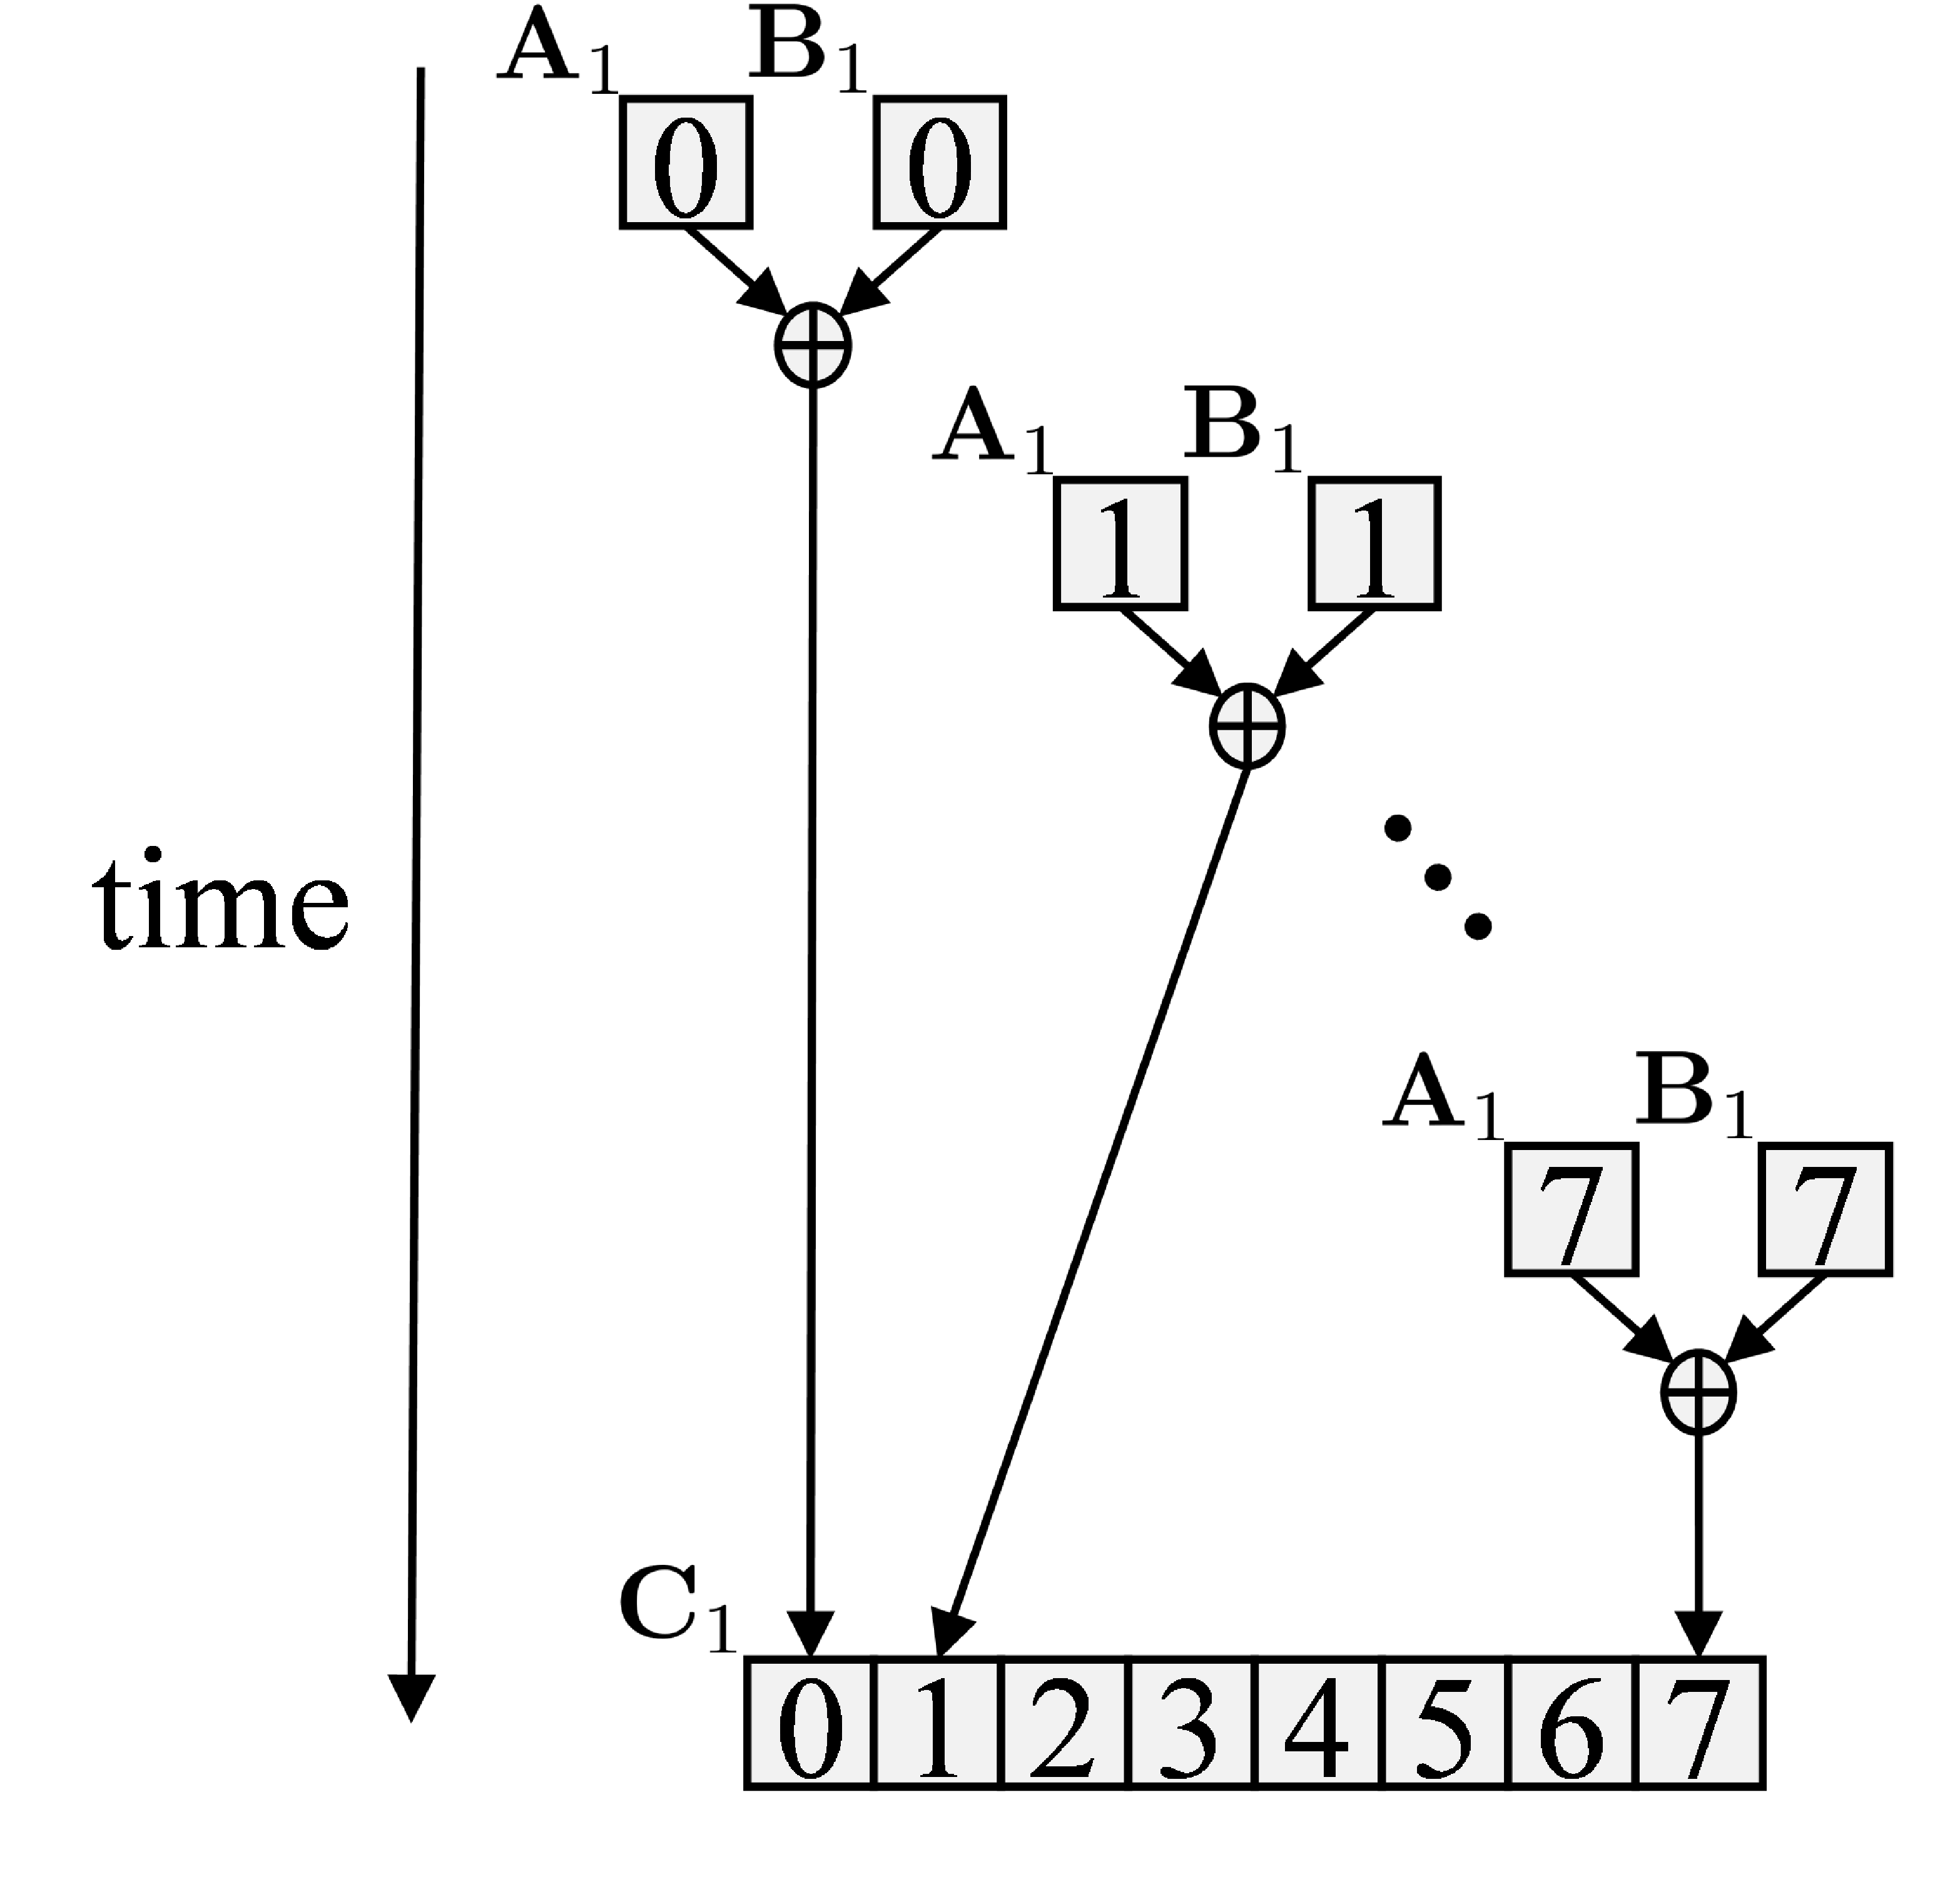
\includegraphics[width=3.17in/100*55]{figures/gpu_intro/CPUaddBlockDiagram.pdf}
	\label{fig:CPUaddBlockDiagram}
	\caption{A block diagram of how a CPU sequentially performs vector addition.}
\end{figure}
\begin{figure}
	\centering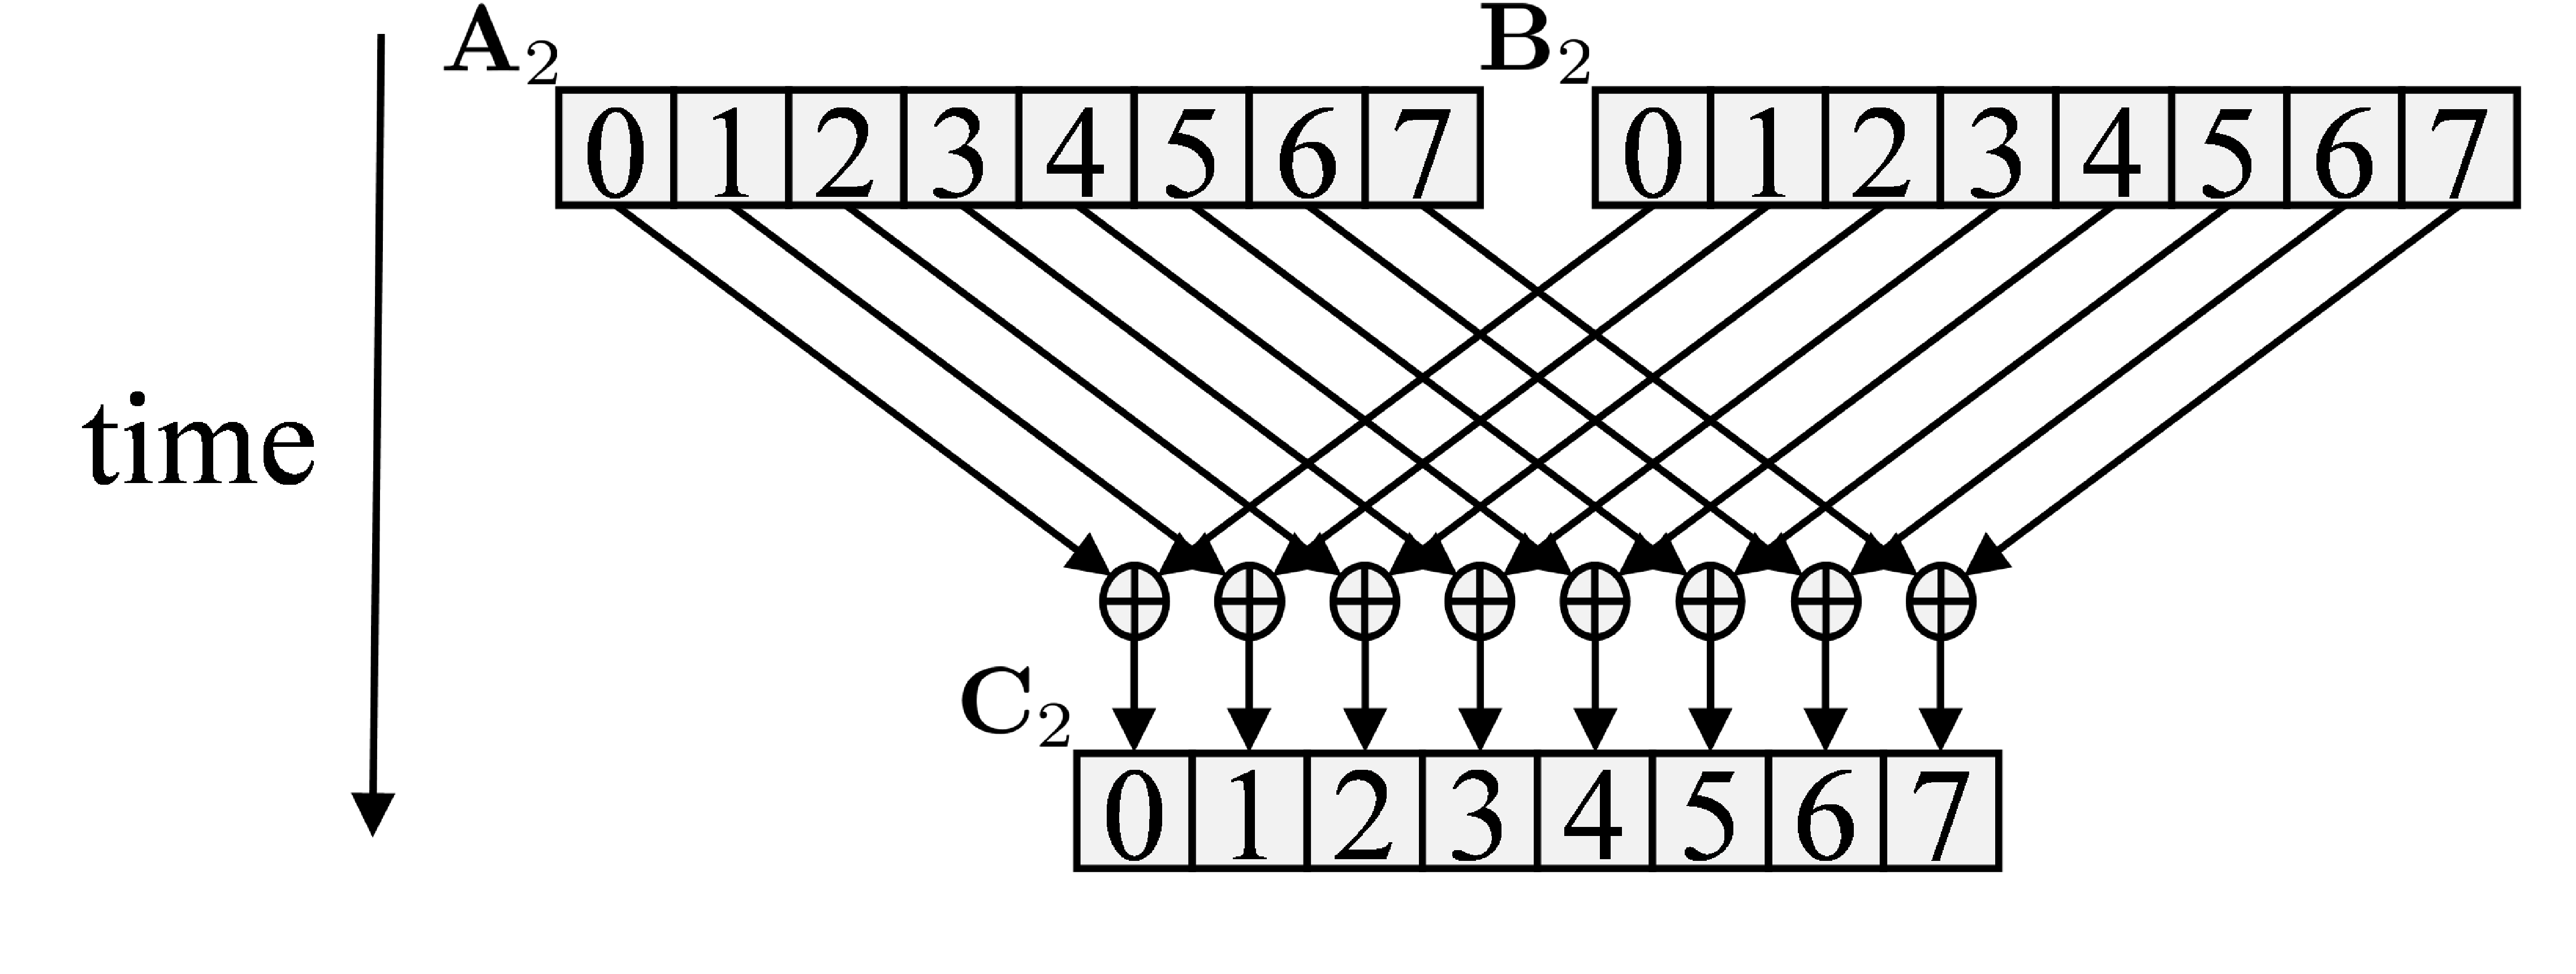
\includegraphics[width=4.69in/100*55]{figures/gpu_intro/GPUaddBlockDiagram.pdf}
	\label{fig:GPUaddBlockDiagram}
	\caption{A block diagram of how a GPU performs vector addition in parallel.}
\end{figure}

\singlespacing
\clearpage
\begin{lstlisting}[style=myCUDAstyle,caption={Comparison of CPU verse GPU code.},label={code:GPUvsCPU}]
#include <iostream>
#include <stdlib.h>
#include <math.h>
using namespace std;

void VecAddCPU(float* destination,float* source0,float* source1,int myLength){
	for(int i = 0; i < myLength; i++)
		destination[i] = source0[i] + source1[i];
}

__global__ void VecAddGPU(float* destination, float* source0, float* source1, int lastThread){
	int i = blockIdx.x*blockDim.x + threadIdx.x;

	// don't access elements out of bounds
	if(i >= lastThread)
		return;

	destination[i] = source0[i] + source1[i];
}

int main(){
	int numPoints = pow(2,22);
	cout << numPoints << endl;
	/**
	* Vector Addition on CPU
	*/
	// allocate memory on host
	float *A1;
	float *B1;
	float *C1;
	A1 = (float*) malloc (numPoints*sizeof(float));
	B1 = (float*) malloc (numPoints*sizeof(float));
	C1 = (float*) malloc (numPoints*sizeof(float));

	// Initialize vectors 0-99
	for(int i = 0; i < numPoints; i++){
		A1[i] = rand()%100;
		B1[i] = rand()%100;
	}

	// vector sum C1 = A1 + B1
	VecAddCPU(C1, A1, B1, numPoints);
	
	/**
	* Vector Addition on GPU
	*/
	// allocate memory on host for result
	float *C2;
	C2 = (float*) malloc (numPoints*sizeof(float));

	// allocate memory on device for computation
	float *A2_gpu;
	float *B2_gpu;
	float *C2_gpu;
	cudaMalloc(&A2_gpu, sizeof(float)*numPoints);
	cudaMalloc(&B2_gpu, sizeof(float)*numPoints);
	cudaMalloc(&C2_gpu, sizeof(float)*numPoints);

	// Copy vectors A and B from host to device
	cudaMemcpy(A2_gpu, A1, sizeof(float)*numPoints, cudaMemcpyHostToDevice);
	cudaMemcpy(B2_gpu, B1, sizeof(float)*numPoints, cudaMemcpyHostToDevice);

	// Set optimal number of threads per block
	int numTreadsPerBlock = 32;

	// Compute number of blocks for set number of threads
	int numBlocks = numPoints/numTreadsPerBlock;

	// If there are left over points, run an extra block
	if(numPoints % numTreadsPerBlock > 0)
		numBlocks++;

	// Run computation on device
	//for(int i = 0; i < 100; i++)
	VecAddGPU<<<numBlocks, numTreadsPerBlock>>>(C2_gpu, A2_gpu, B2_gpu, numPoints);

	// Copy vector C2 from device to host
	cudaMemcpy(C2, C2_gpu, sizeof(float)*numPoints, cudaMemcpyDeviceToHost);

	// Compare C2 to C1
	bool equal = true;
	for(int i = 0; i < numPoints; i++)
		if(C1[i] != C2[i])
			equal = false;
	if(equal)
		cout << "C2 is equal to C1." << endl;
	else
		cout << "C2 is NOT equal to C1." << endl;

	// Free vectors on CPU
	free(A1);
	free(B1);
	free(C1);
	free(C2);

	// Free vectors on GPU
	cudaFree(A2_gpu);
	cudaFree(B2_gpu);
	cudaFree(C2_gpu);
}
\end{lstlisting}
\doublespacing

\section{GPU kernel using threads and thread blocks}
A GPU kernel is executed on a GPU by launching numBlocks thread blocks with a set number of threads per block.
In the Listing \ref{code:GPUvsCPU}, VecAddGPU is launched with $32$ threads per block on line $75$.
The total number of threads launched on the GPU is the number of blocks times the number of threads per block.
VecAddGPU needs to be launched with atleast $2^22$ threads or $131072 = 2^22/32$ blocks of $32$ threads.

CUDA gives each thread launched in a GPU kernel a unique index called threadIdx and blockIdx.
threadIdx is the thread index inside the assigned thread block.
blockIdx is the index of the block that the thread is assigned to.
blockDim is the number of threads assigned per block, in fact blockDim $=$ numTreadsPerBlock.
Both threadIdx and blockIdx are three dimensional and have x, y and z components.
In this thesis only the x dimension is used because GPU kernels operate only on one dimensional vectors.

To turn a CPU for loop in to a GPU kernel that runs $0$ to $N-1$, the GPU kernel will launch atleast $N$ threads are with $T$ threads per thread block.
The number of blocks need is $M = \frac{N}{T}$ or $M = \frac{N}{T}+1$ if $N$ is not an integer multiple of $T$.
Figure \ref{fig:threadsBlocks32} shows $32$ threads launched in $4$ thread blocks with $8$ threads per block.
Figure \ref{fig:threadsBlocks36} shows $36$ threads launched in $5$ thread blocks with $8$ threads per block. 
An full extra thread block is launched with $8$ threads but $4$ threads are idle.
\begin{figure}
	\centering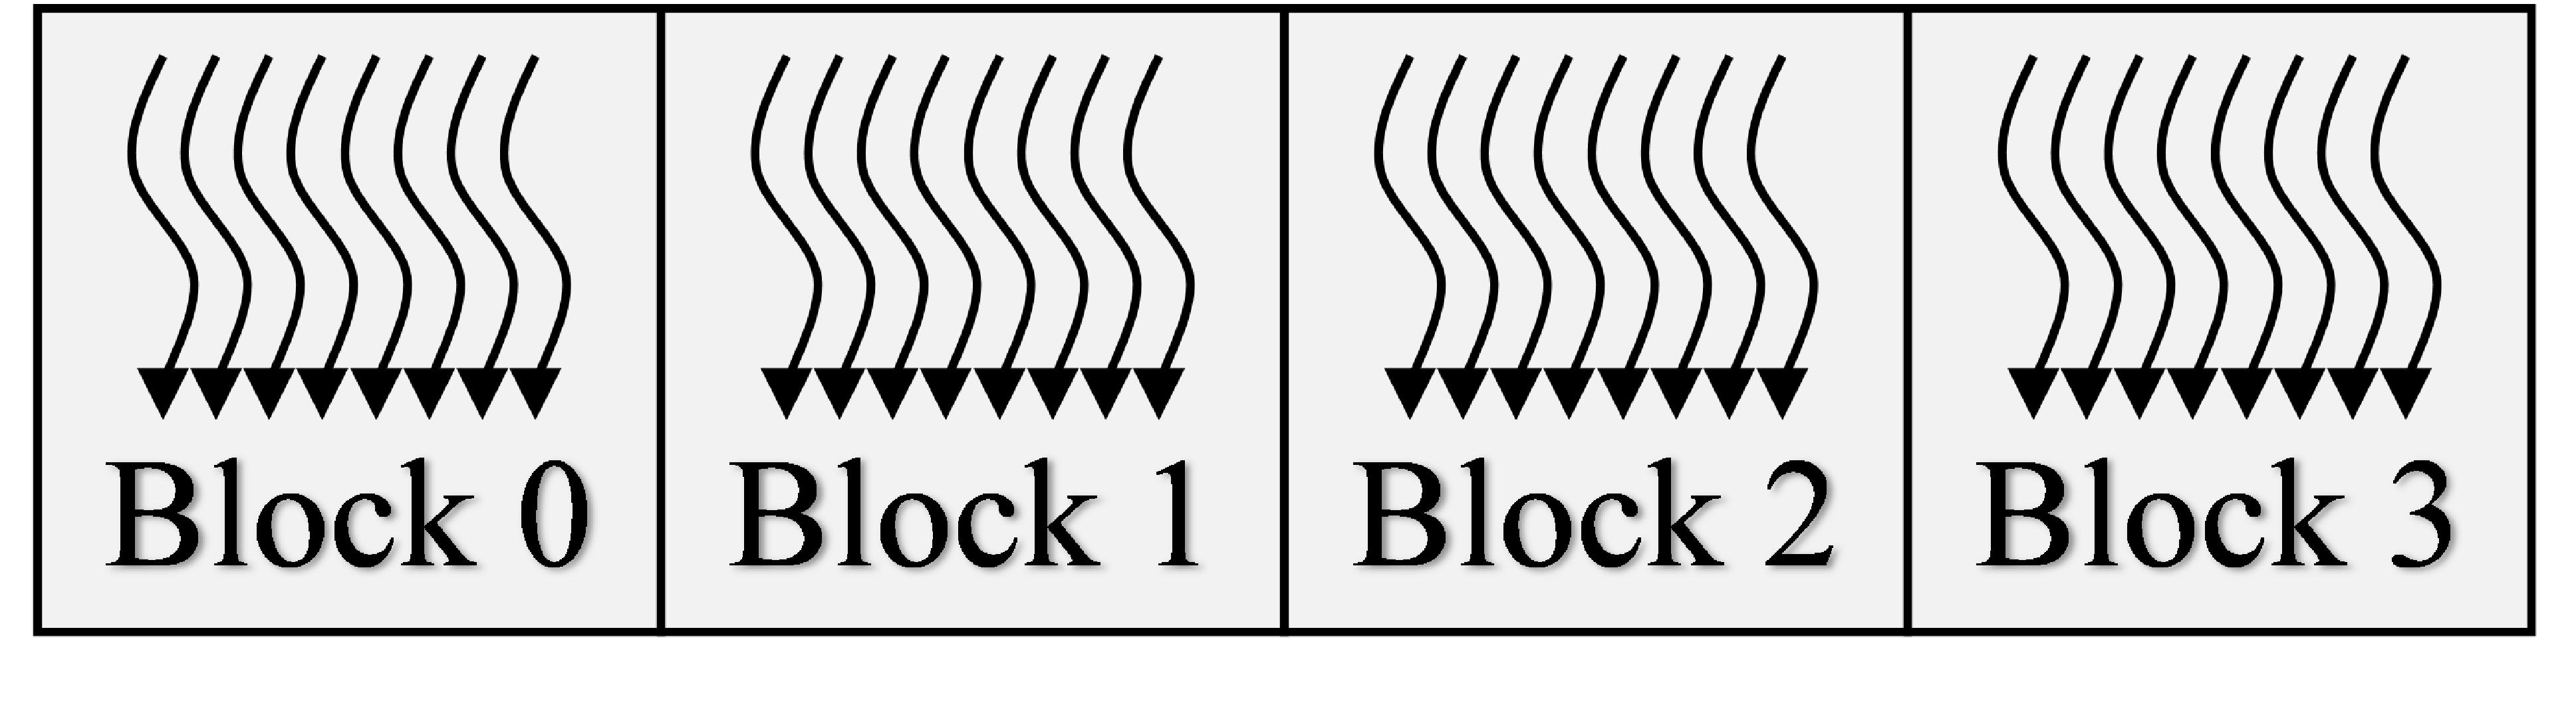
\includegraphics[width=4in/100*55]{figures/gpu_intro/threadsBlocks32.pdf}
	\label{fig:threadsBlocks32}
	\caption{Block $0$ $32$ threads launched in $4$ thread blocks with $8$ threads per block.}
\end{figure}
\begin{figure}
	\centering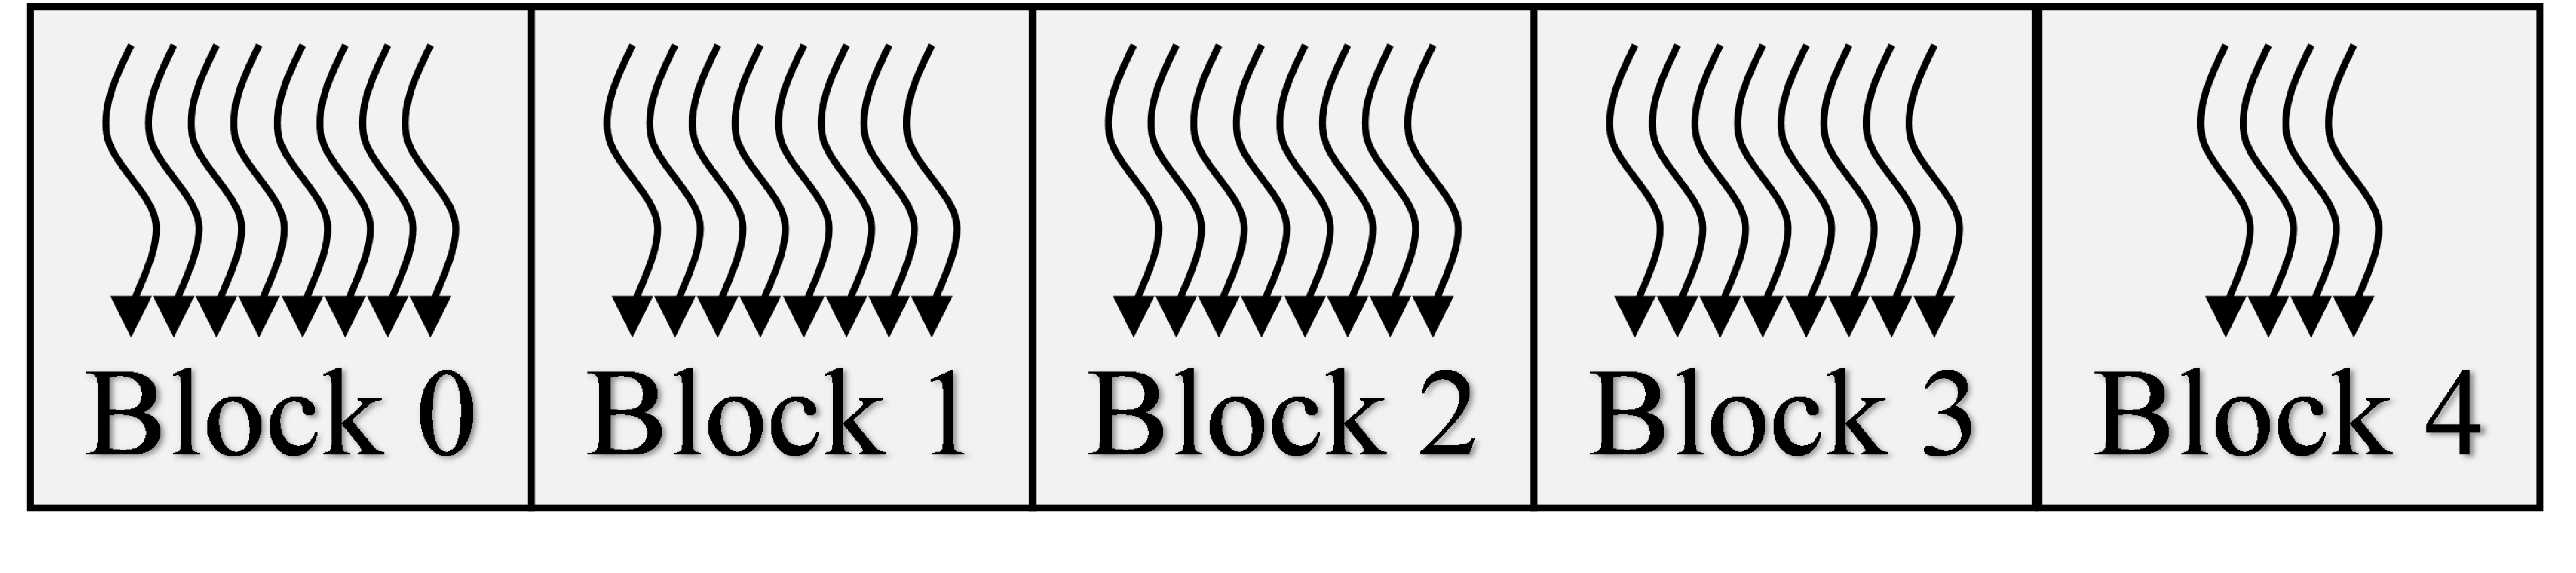
\includegraphics[width=5in/100*55]{figures/gpu_intro/threadsBlocks36.pdf}
	\label{fig:threadsBlocks36}
	\caption{$36$ threads launched in $5$ thread blocks with $8$ threads per block with $4$ idle threads.}
\end{figure}

\section{GPU Execution and Memory}
\label{sec:GPU_memory}
Thread blocks are executed independent of other thread blocks.
The GPU does not guarantee Block $0$ will execute before Block $2$.
Threads in individual blocks can coordinate and use shared memory but blocks do not coordinate with other blocks.
Threads have access to private local memory that is fast and efficient.
Each thread in a thread block has access to shared memory the is private to the thread block.
All threads have access to global memory.

Local memory is the fastest and global memory is by far the slowest.
One global memory access takes 400-800 clock cycles while a local memory in the form of registers, L1 and shared memory is a few clock cycles.
Figure \ref{fig:MemoryPyramid} helps visualize the trade offs of memory and 
Figure \ref{fig:fullGPUmemBlockDiagram} shows where each type of memory is located.
\begin{figure}
	\centering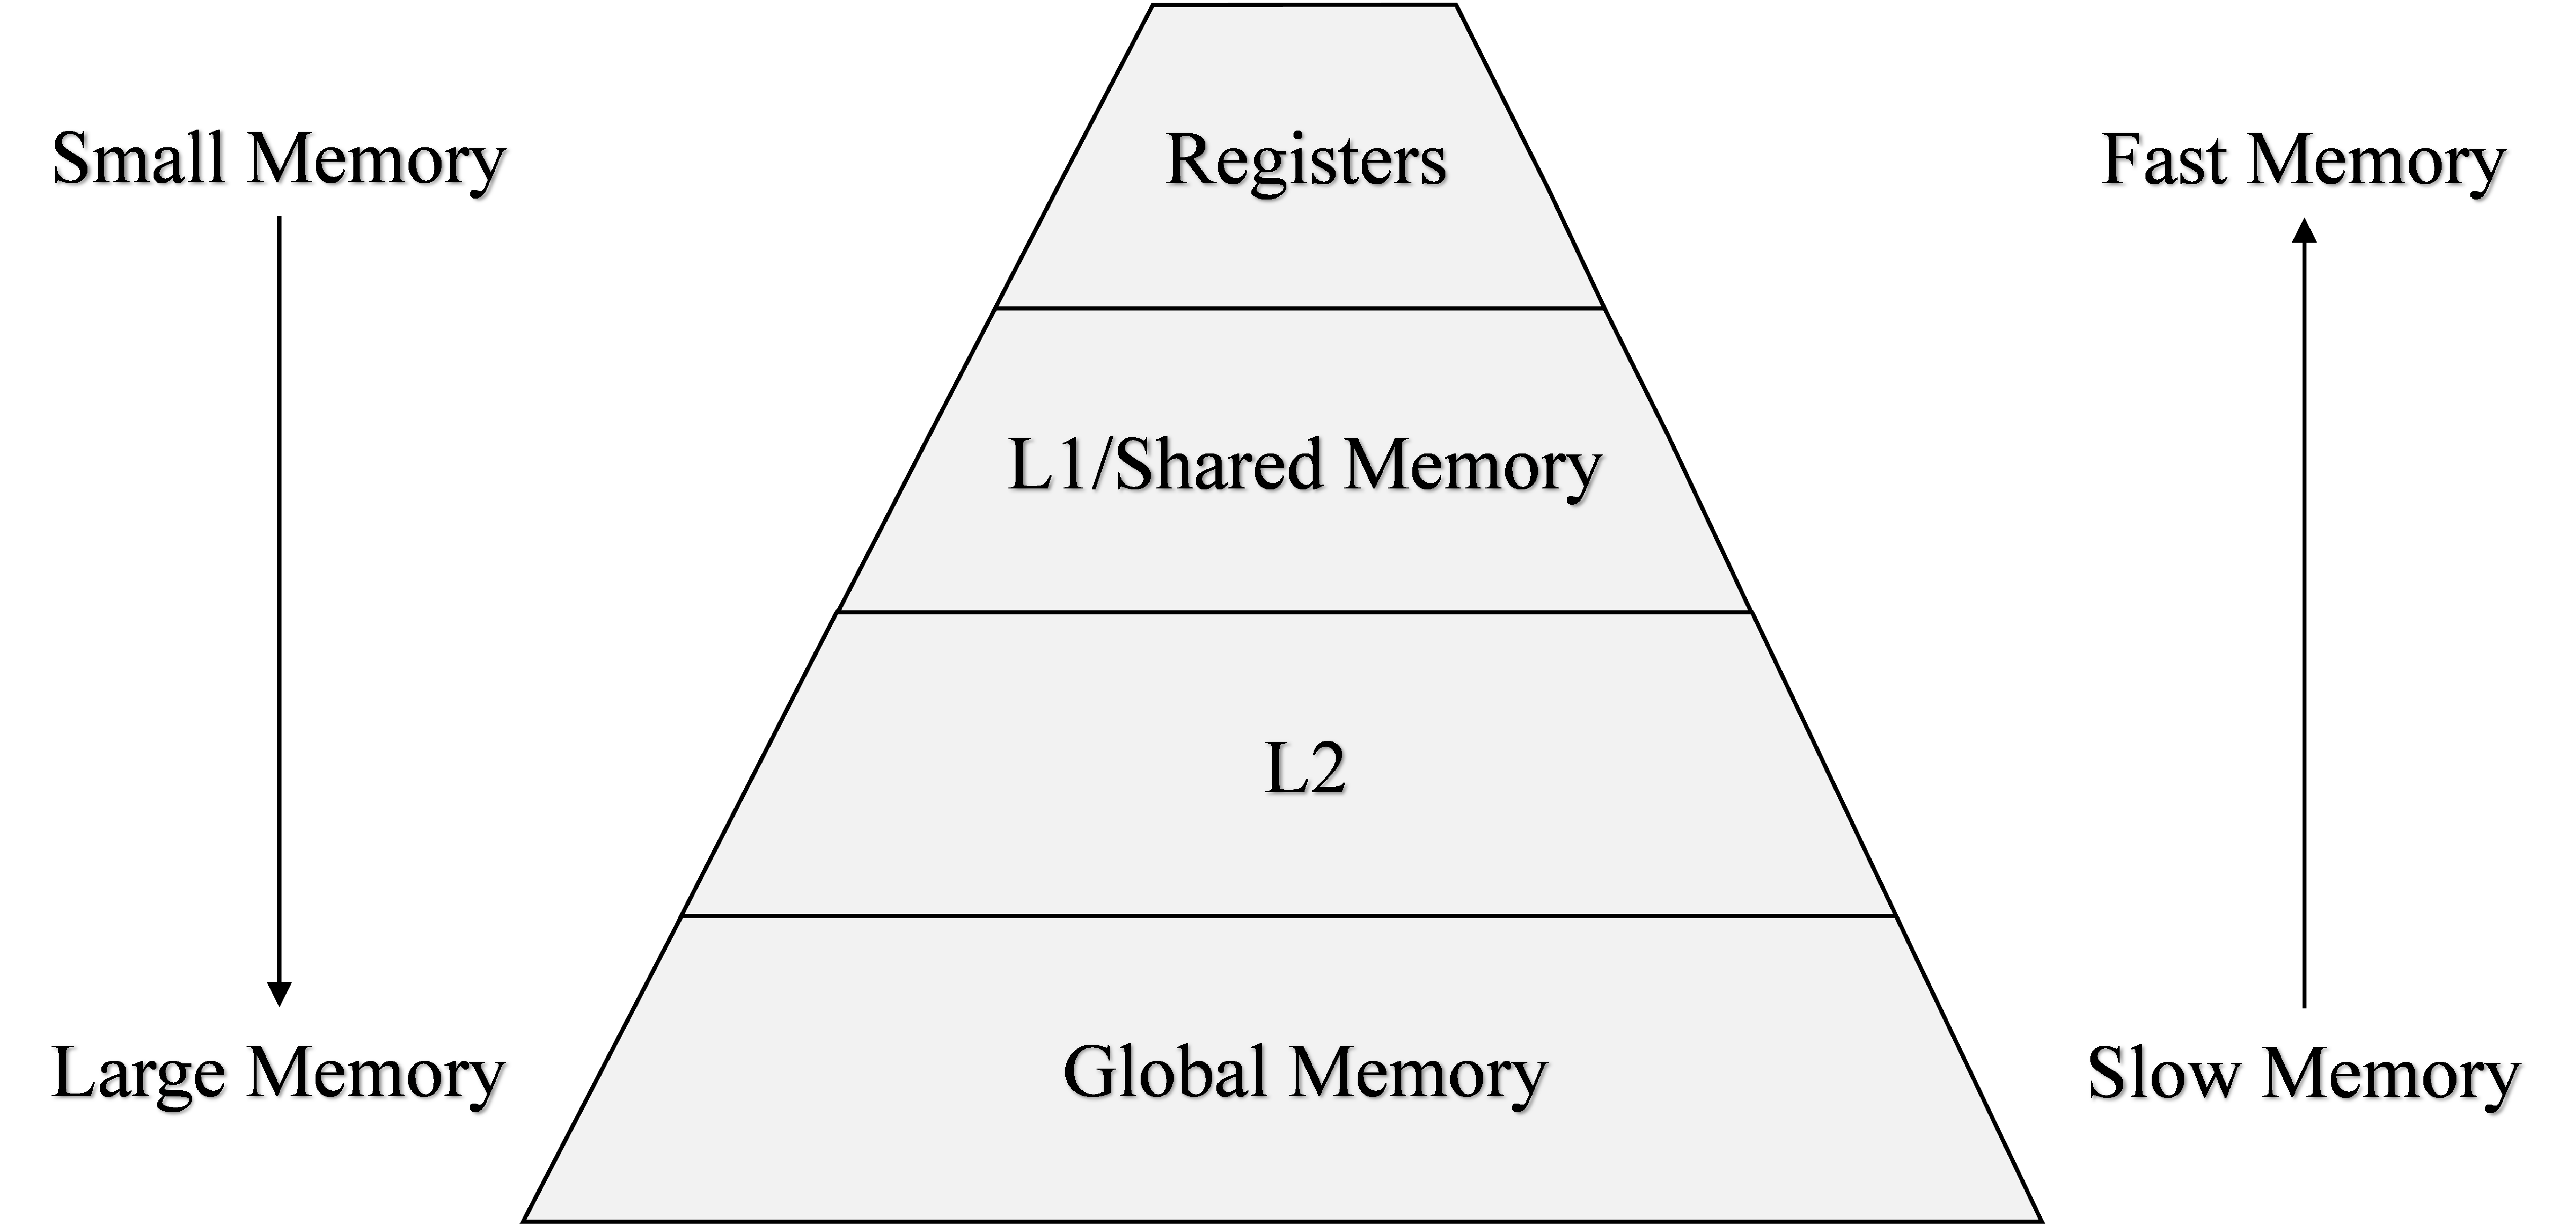
\includegraphics[width=8.36in/100*55]{figures/gpu_intro/MemoryPyramid.pdf}
	\label{fig:MemoryPyramid}
	\caption{Diagram comparing memory size and speed. Global memory is massive but extremely slow. Registers are extremely fast but there are very few.}
\end{figure}
\begin{figure}
	\centering\includegraphics[width=9.83in/100*55]{figures/gpu_intro/fullGPUmemBlockDiagram.pdf}
	\label{fig:fullGPUmemBlockDiagram}
	\caption{A block diagram where local, shared, and global memory is located. Each thread has private local memory. Each thread block has private shared memory. The GPU has global memory that all threads can access.}
\end{figure}

Why not just use local memory for all computation storage?
Elements need to come from global memory to before they can be used in local memory.
If many threads access the same elements in global memory, clock cycles can be saved by copying the elements from global to shared memory.
Local and shared memory should be used as much as possible but sometimes a GPU kernel cant utilized local and shared memory because elements might only be used once.


Why is global memory so slow?
Looking at the physical hardware is instructive.
This thesis uses NVIDIA Tesla K40c and K20c GPUs, Table \ref{tab:gpu-resources_jeffs} lists some specifications and Figure \ref{fig:GPUpicture} shows the form factor of the these GPUs.
The red box in Figure \ref{fig:GPUarch} shows the GPU chip and the yellow boxes show the SRAM that is \textit{off} the GPU chip.

The global memory is located in the SRAM.
To move memory to thread blocks \textit{on} the GPU chip from global memory requires fetching memory from \textit{off} the GPU.
Considering that global memory is off chip, 400-800 clock cycles doesn't sound all that bad.
\begin{figure}
	\centering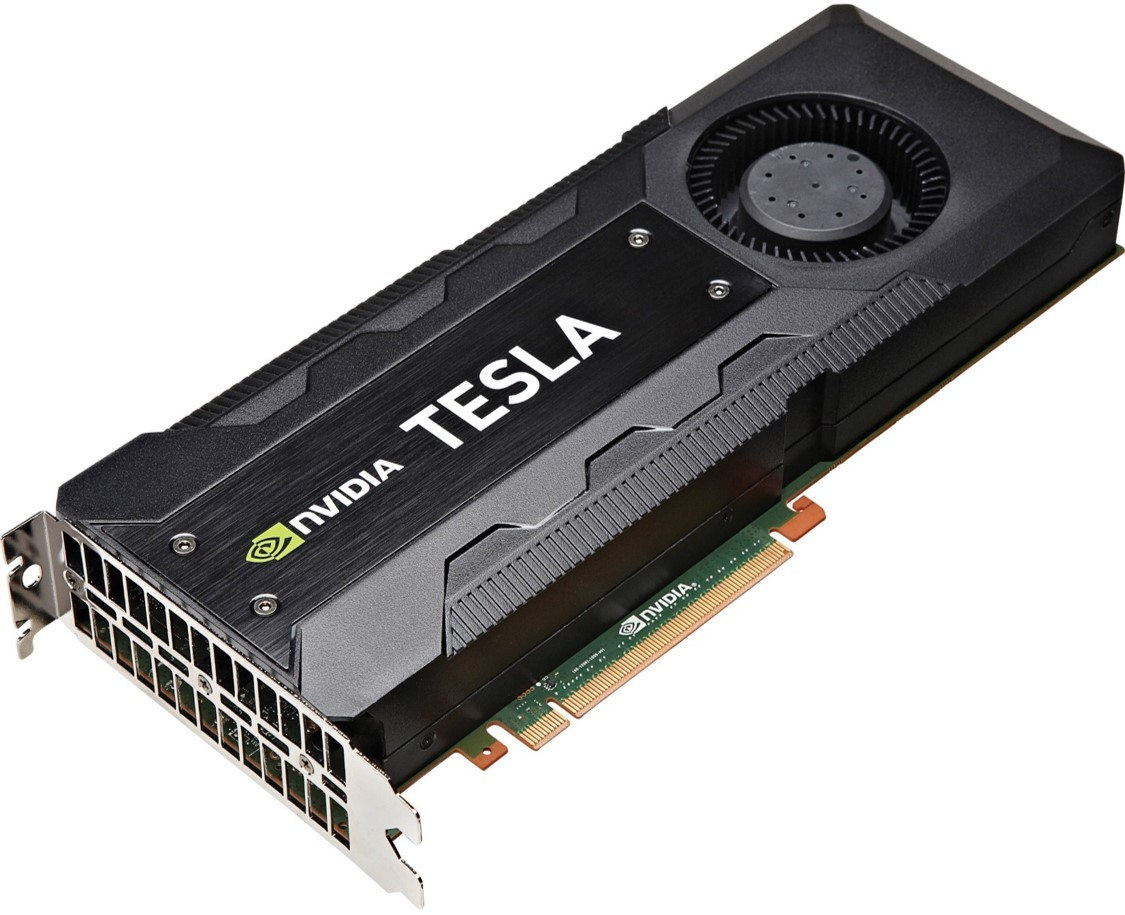
\includegraphics[width=5in]{figures/gpu_intro/k40c_k20c.jpg}
	\label{fig:GPUpicture}
	\caption{NVIDIA Tesla K40c and K20c.}
\end{figure}
\begin{figure}
	\centering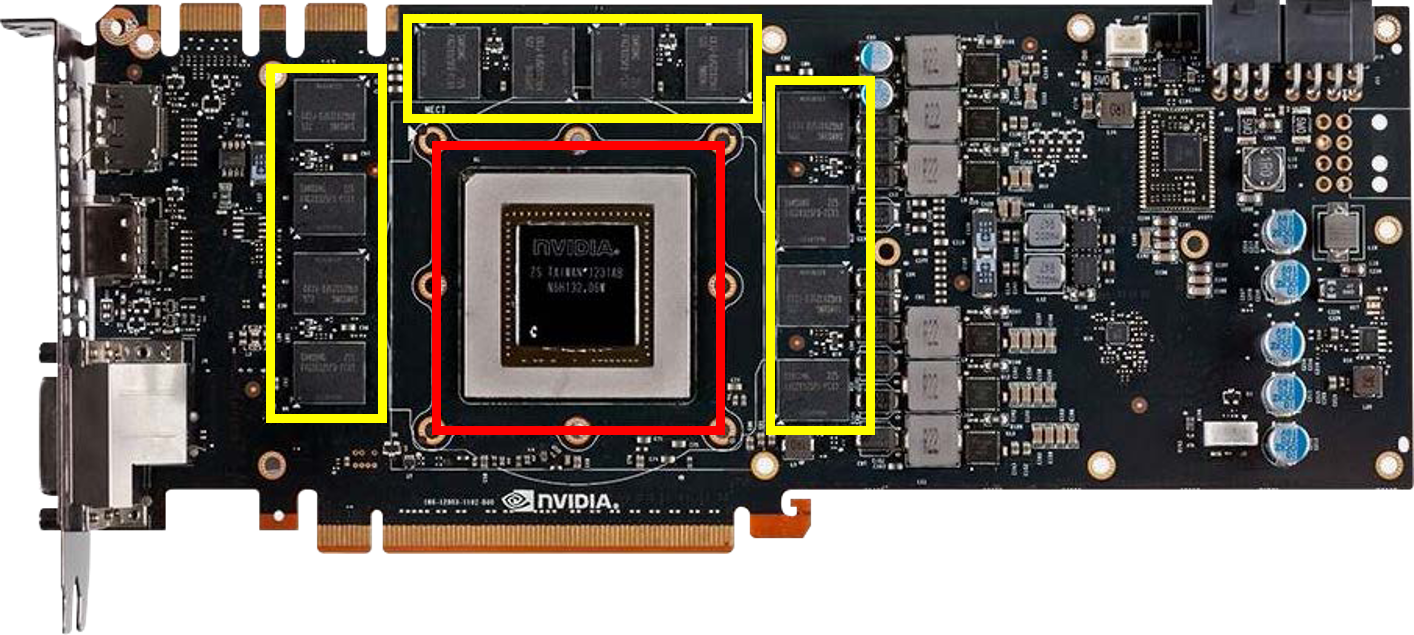
\includegraphics[width=\textwidth]{figures/gpu_intro/Kepler_box.png}
	\label{fig:GPUarch}
	\caption{Example of an NVIDIA GPU card. The SRAM is shown to be boxed in yellow. The GPU chip is shown to be boxed in red.}
\end{figure}
\begin{table}
\begin{center}
\begin{tabular}{lll}
	\toprule
	Feature 			& Tesla K40c 	& Tesla K20c 	\\ \midrule
	Memory size (GDDR5) & 12 GB 		& 5 GB 			\\
	CUDA cores 			& 2880 			& 2496 			\\
	Base clock (MHz) 	& 745 			& 732 			\\ \bottomrule
\end{tabular}
\end{center}
\label{tab:gpu-resources_jeffs}
\caption{The computational resources available with three NVIDIA GPUs used in this thesis (1x Tesla K40c 2x Tesla K20c).}
\end{table}

\section{Thread Optimization}
When writing a custom GPU kernel, it is tempting to launch as many threads per block as possible.
Launching 256 threads per block doesn't sound as fast at launching 1024 threads per block, right?
Wrong. Running the GPU at low occupancy provides each thread with more resources in the each block.
Running the GPU at high occupancy provides each thread with less resources.

Launching 1024 threads per block isnt always bad though.
1024 might be the optimal number of threads per block.
If a GPU kernel was very computationally heavy but didn't require much memory resources, 1024 threads might be a good amount of threads per block.

Improving memory accesses should always be the first optimization when a GPU kernel needs to be faster.
The next step is to find the optimal number of threads per block to launch.
Knowing the perfect number of threads per block to launch is challenging to calculate.
Luckily, there is a finite number of possible threads per block, $1$ to $1024$.
Listing \ref{code:threadTiming} shows a simple test program that times GPU kernel execution time while sweeping the number of possible threads per block.
The number of threads per block with the fastest computation time is the optimal number of threads per block for that specific GPU kernel.

\singlespacing
\clearpage
\begin{lstlisting}[style=myCUDAstyle,caption={Code snippet for thread optimization.},label={code:threadTiming}]
float milliseconds_opt = pow(2,10); // initiaize to "big" number
int numTreadsPerBlock_opt;
int minNumTotalThreads = pow(2,20); // set to minimum number of required threads
for(int numTreadsPerBlock = 1; numTreadsPerBlock<=1024; numTreadsPerBlock++){
	int numBlocks = minNumTotalThreads/numTreadsPerBlock;
	if(minNumTotalThreads % numTreadsPerBlock > 0)
		numBlocks++;
	cudaEvent_t start, stop;
	cudaEventCreate(&start);
	cudaEventCreate(&stop);
	cudaEventRecord(start);
	
	GPUkernel<<<numBlocks, numTreadsPerBlock>>>(dev_vec0, dev_vec1);
	
	cudaEventRecord(stop);
	cudaEventSynchronize(stop);
	float milliseconds = 0;
	cudaEventElapsedTime(&milliseconds, start, stop);
	cudaEventDestroy(start);
	cudaEventDestroy(stop);
	if(milliseconds<milliseconds_opt){
		milliseconds_opt = milliseconds;
		numTreadsPerBlock_opt = numTreadsPerBlock;
	}
}
cout << "Optimal Threads Per Block " << numTreadsPerBlock_opt << endl
cout << "Optimal Execution Time    " << milliseconds_opt      << endl;
\end{lstlisting}
\doublespacing

Most of the time the optimal number of threads per block is a multiple of $32$. 
At the lowest level of architecture, GPUs do computations in \textit{warps}.
Warps are groups of $32$ threads that do every computation together in lock step.
If the number of threads per block is a non multiple of $32$, some threads in a warp will be idle and the GPU will have unused resources.


Figure \ref{fig:ConvGPU_shared_12672_186taps} shows the execution time of an example GPU kernel
The optimal execution time is $0.1078$ms at the optimal $96$ threads per block.
By simply adjusting the number of threads per block, this example kernel can have a $2\times$ speed up.

Adjusting the number of threads per block doesn't always drastically speed up GPU kernels.
Figure \ref{fig:ConvGPU_shared_12672_186taps} shows the execution time for another GPU kernel with varying threads per block.
Launching $560$ does produce about a $1.12\times$ speed up.
\begin{figure}
	\centering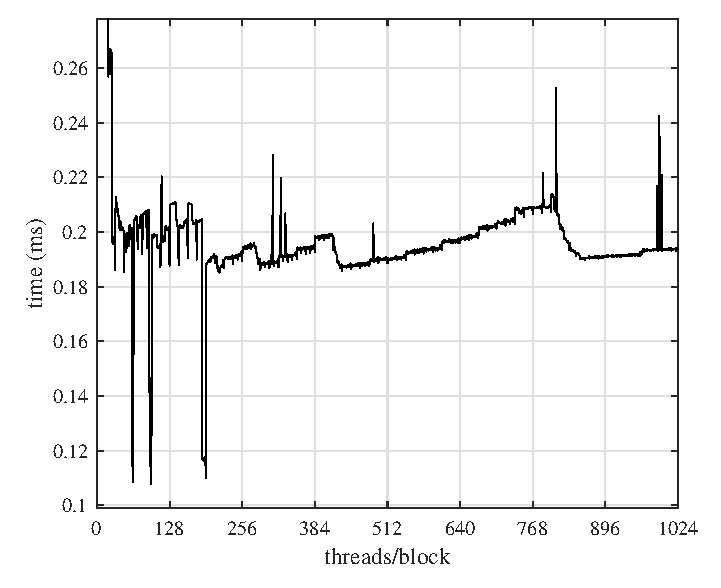
\includegraphics[width=5in]{figures/gpu_intro/ConvGPU_shared_12672_186taps.eps}
	\label{fig:ConvGPU_shared_12672_186taps}
	\caption{Plot showing how execution time is affected by changing the number of threads per block.
	The optimal execution time for an example GPU kernel is $0.1078$ms at the optimal $96$ threads per block.}
\end{figure}
\begin{figure}
	\centering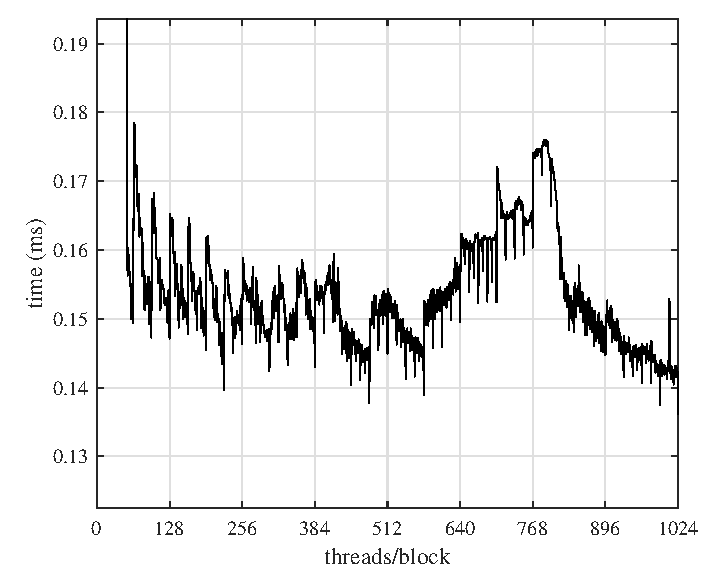
\includegraphics[width=5in]{figures/gpu_intro/ConvGPU_global_12672_186taps.eps}
	\label{fig:ConvGPU_global_12672_186taps}
	\caption{Plot showing the number of threads per block doesn't always drastically affect execution time.}
\end{figure}
%Figure \ref{fig:ConvGPU_shared_12672_186taps} shows the execution time of ConvGPUshared from Listing \ref{code:convFun} while varying threads per block.
%Although the minimum execution time is $0.1078$ms at the optimal $96$ threads per block, but ConvGPUshared must be lauched with atleast $186$ threads per block because of the way the kernel uses shared memory.
%Luckily, launching $192$ threads per block is near optimal with an execution time of $0.1101$ms.
%By simply adjusting the number of threads per block, ConvGPUshared can have a $2\times$ speed up.
%
%Adjusting the number of threads per block doesn't always drastically speed up GPU kernels.
%Figure \ref{fig:ConvGPU_shared_12672_186taps} shows the execution time for ConvGPU with varying threads per block.
%Launching $560$ does produce about a $1.12$x speed up, but thread optimization doesn't have as much of an affect of ConvGPU verse ConvGPUshared.
%\begin{figure}
%	\centering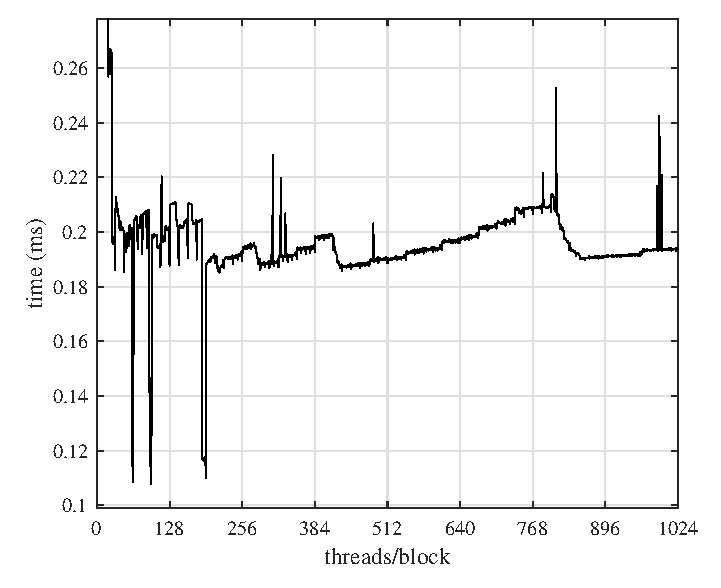
\includegraphics[width=5in]{figures/gpu_intro/ConvGPU_shared_12672_186taps.eps}
%	\label{fig:ConvGPU_shared_12672_186taps}
%	\caption{The GPU convolution thread optimization of a $12672$ length signal with a $186$ tap filter using shared memory. $192$ is the optimal number of threads per block executing in $0.1101$ms. Note that at least $186$ threads per block must be launched to compute correct output.}
%\end{figure}
%\begin{figure}
%	\centering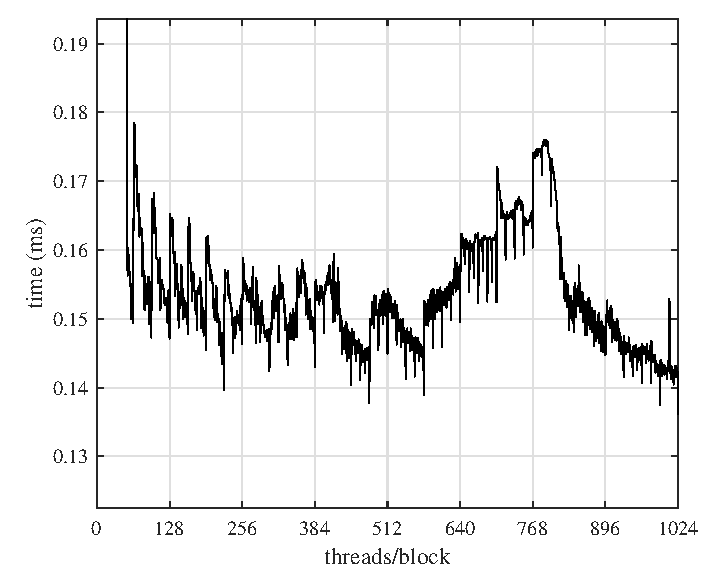
\includegraphics[width=5in]{figures/gpu_intro/ConvGPU_global_12672_186taps.eps}
%	\label{fig:ConvGPU_global_12672_186taps}
%	\caption{ConvGPU thread optimization 128 threads per block 0.006811.}
%\end{figure}
%To answer the question: ``There are $X$ number of ways to implement this algorithm, which one is executes the fastest?'' the answer always is ``It depends. Implement the algorithm $X$ ways and see which is fastest.''

%\section{Cuda Libraries}
While writing a custom GPU kernel then figuring out how to optimize it is extremely satisfying,
CUDA has super optimized GPU libraries that are extremely useful and efficient.
The CUDA libraries are written by NVIDIA engineers that know how to squeeze out every drop of performance out of NVIDIA GPUs.
Some libraries used in this thesis are cuFFT, cuBLAS and cuSolverSp.

\section{CPU GPU Pipelining}
A basic program flow is shown in Listing \ref{code:noPipe}.
The CPU acquires data from myADC on Line 5.
After taking time to acquire data, the data is copied to the CPU, the data is processed in the GPU then result is copied back to the CPU on Lines $8$ to $10$.
cudaDeviceSynchronize on line $13$ causes the CPU to wait until all instructions on the GPU are complete.
Acquiring and copying data takes precious processing time.
What if the GPU could be processing data while the CPU acquires and copied data?
How much computation time could be gained by pipelining acquiring data and processing data?
How much would the throughput increase?

Figure \ref{fig:concurrentCPU_nonBlocking} shows a block diagram of what is happening on the CPU and GPU in Listing \ref{code:noPipe}.
The GPU is idle while the CPU is acquiring data.
The CPU is idle while the GPU is processing and data is being transferred to and from the GPU.
\begin{figure}
	\centering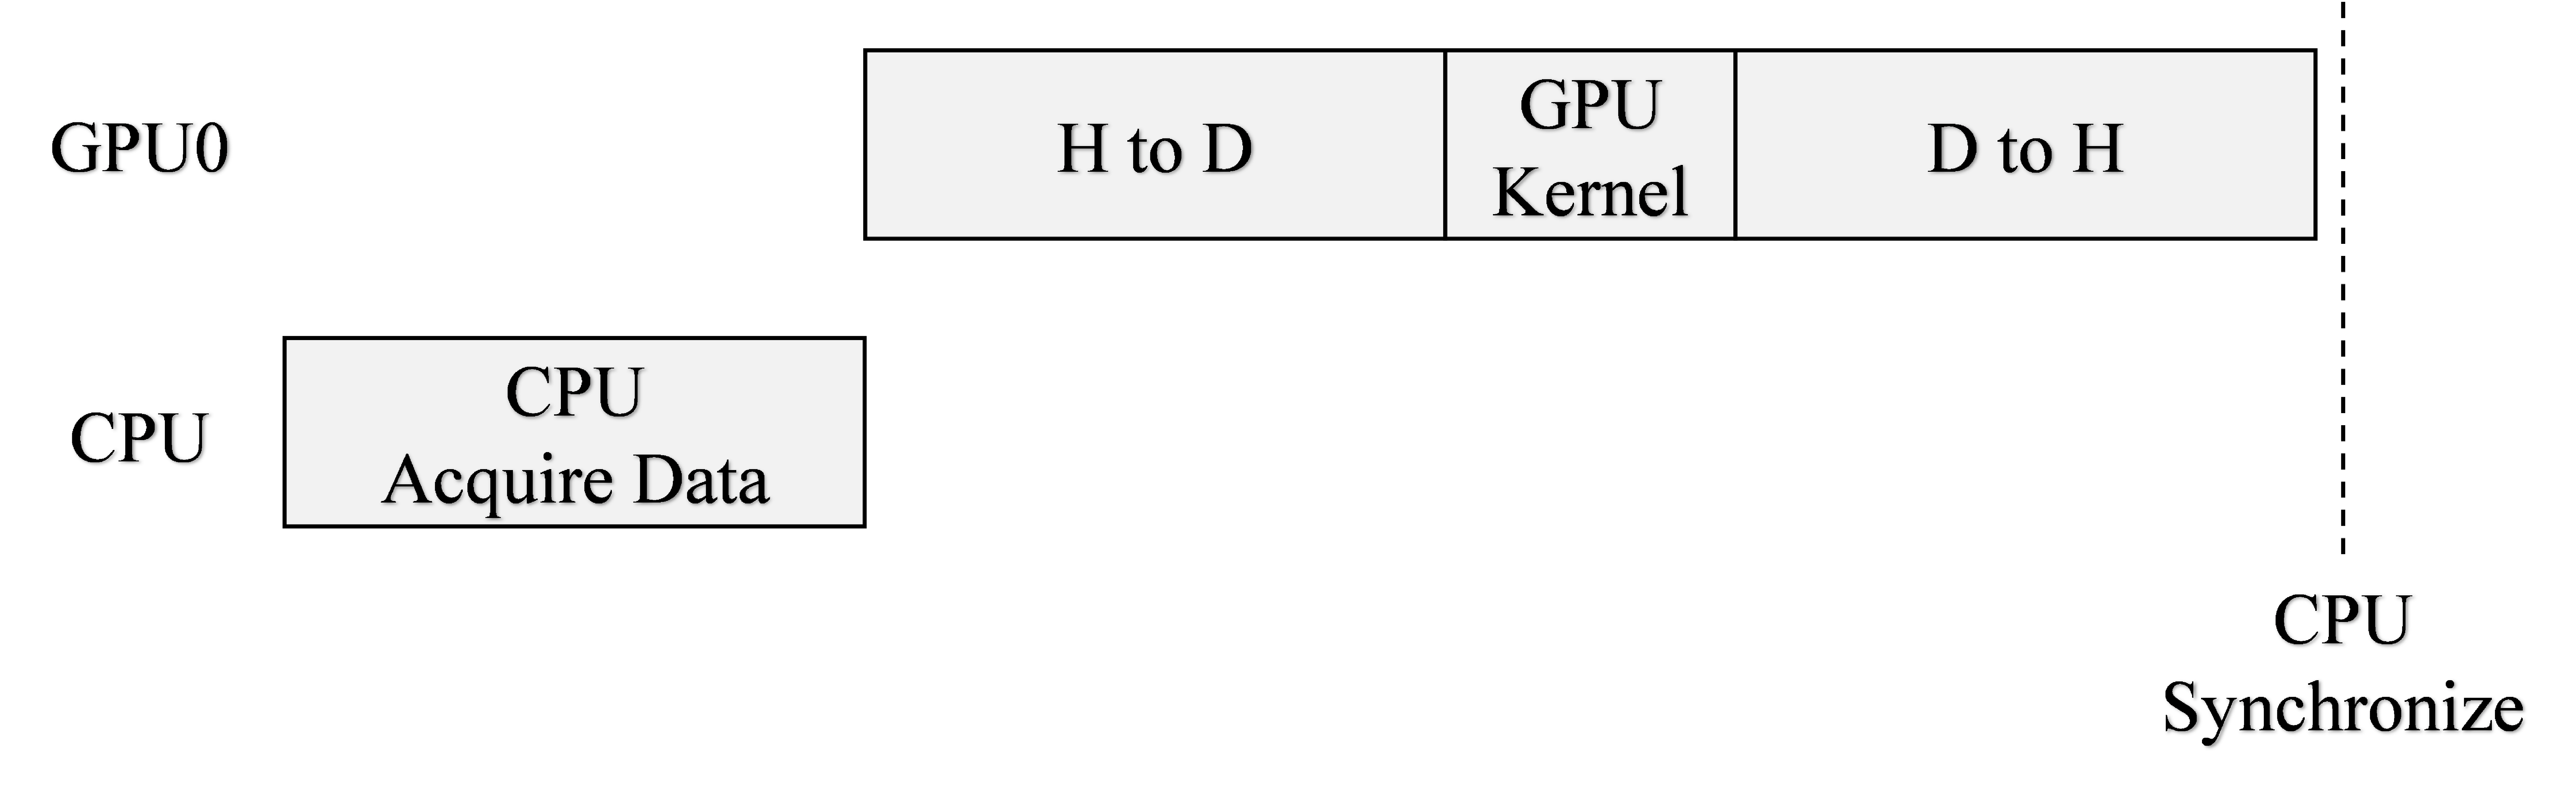
\includegraphics[width=8.77in/100*55]{figures/gpu_intro/concurrentCPU_nonBlocking.pdf}
	\label{fig:concurrentCPU_nonBlocking}
	\caption{The typical approach of CPU and GPU operations. This block diagram shows the profile of Listing \ref{code:noPipe}.}
\end{figure}

\clearpage
\singlespacing
\begin{lstlisting}[style=myCUDAstyle,caption={Example code Simple example of the CPU acquiring data from myADC, copying from host to device, processing data on the device then copying from device to host. No processing occurs on device while CPU is acquiring data.},label={code:noPipe}]
int main()
{
	...
	// CPU Acuire Data
	myADC.acquire(vec);
	
	// Launch instructions on GPU 
	cudaMemcpy(dev_vec0, vec,      numBytes, cudaMemcpyHostToDevice);
	GPUkernel<<<1, N>>>(dev_vec0);
	cudaMemcpy(vec,      dev_vec0, numBytes, cudaMemcpyDeviceToHost);
	
	// Synchronize CPU with GPU
	cudaDeviceSynchronize();
	...
}
\end{lstlisting}
\doublespacing

Can the throughput increase by using idle time on the GPU and CPU?
Yes, CPU and GPU operations can sacrifice latency for throughput by pipelineing.
After the CPU gives instructions to the GPU, the CPU can do other operations like acquire data or perform algorithms better suited for CPUs than the GPUs.
Once the CPU has finished its operations, the CPU can wait for the GPU to finish.

Listing \ref{code:pipe} shows how to pipeline CPU and GPU operations.
Assuming data is already on the GPU from a prior iteration, the CPU gives instructions to the GPU then starts acquiring data.
The CPU then does an asynchronous data transfer to a temporary vector on the GPU.
The GPU first performs a device to device transfer from the temporary vector.
The GPU then runs the GPUkernel and transfers the result to the host.
This system suffers a full cycle latency.
\begin{figure}
	\centering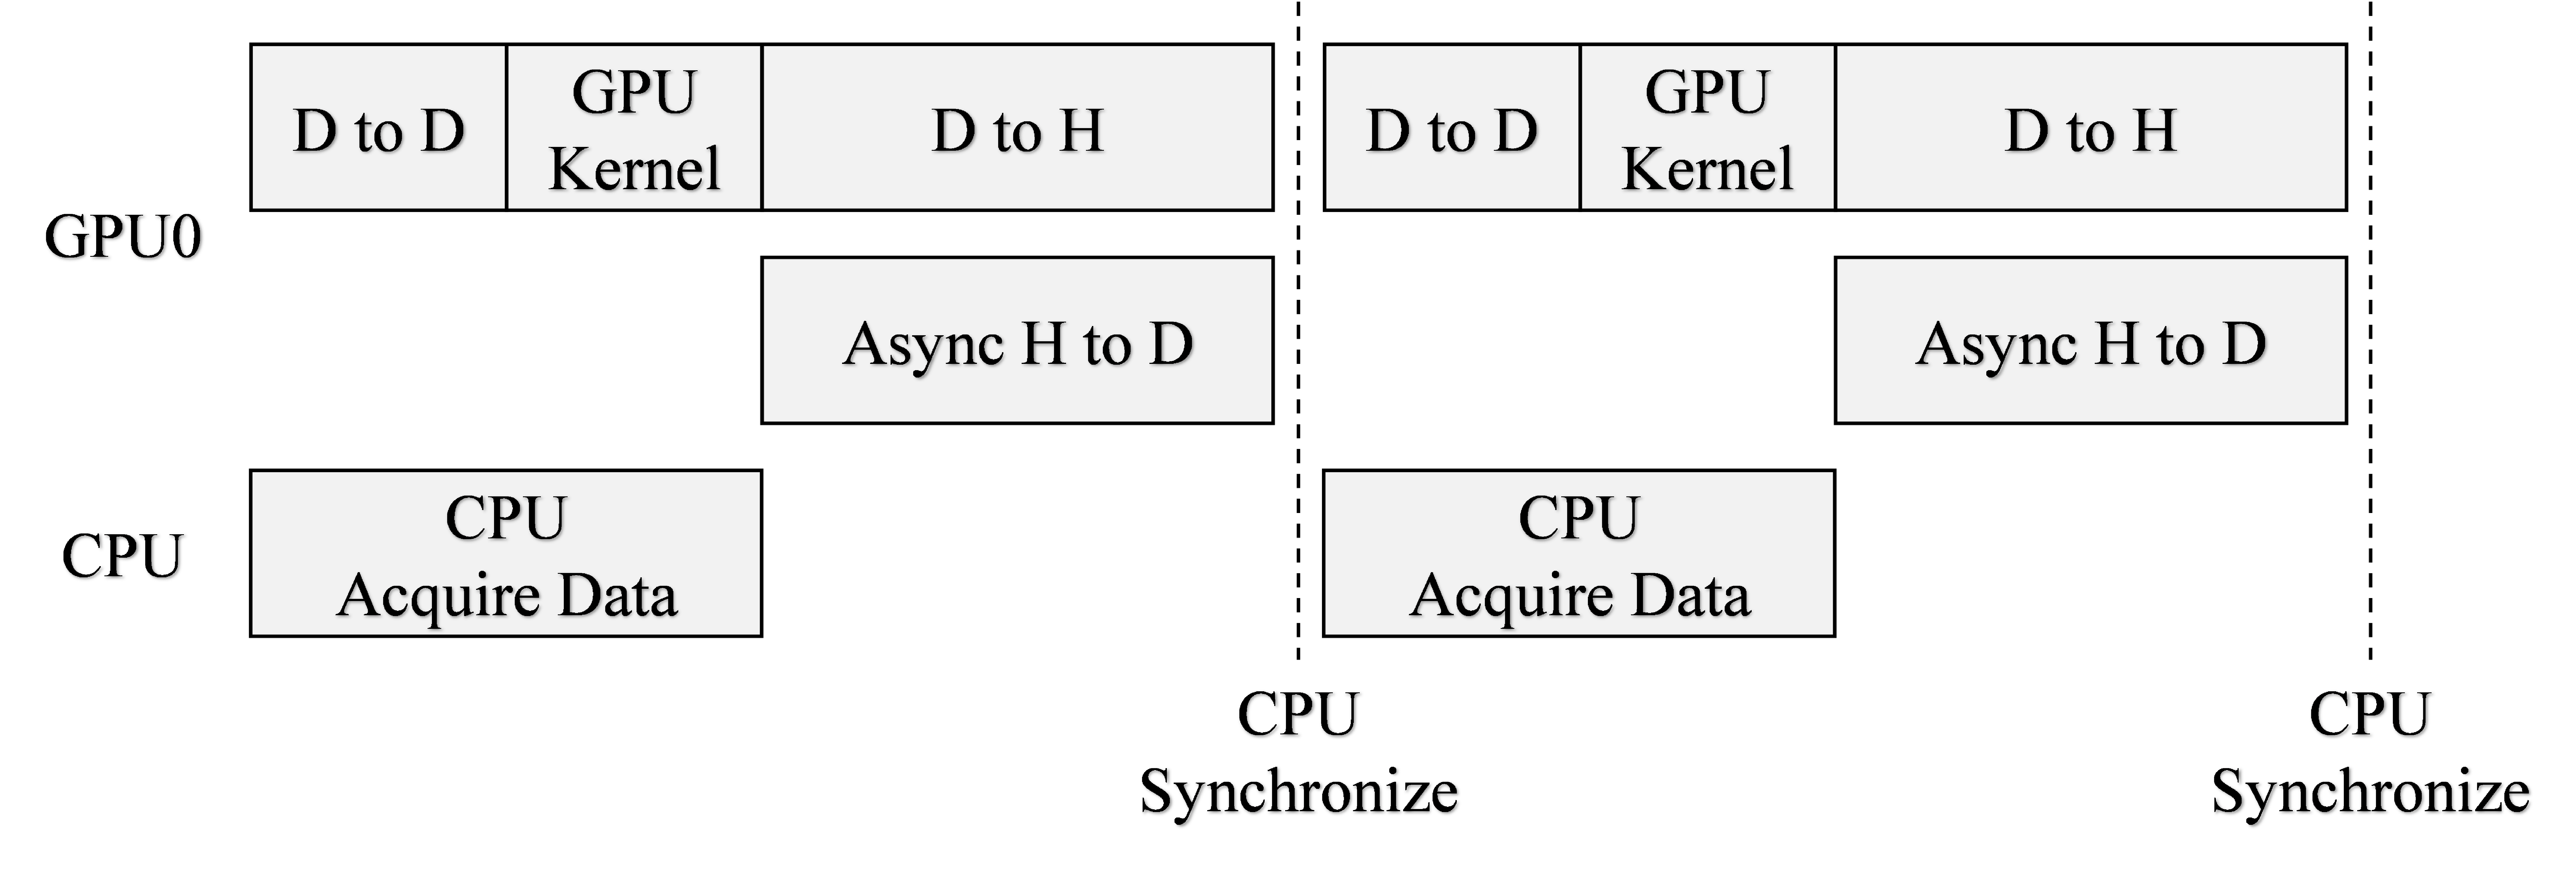
\includegraphics[width=9.97in/100*55]{figures/gpu_intro/concurrentCPU_blocking.pdf}
	\label{fig:concurrentCPU_blocking}
	\caption{GPU and CPU operations can be pipelined. This block diagram shows a Profile of Listing \ref{code:pipe}.}
\end{figure}

\singlespacing
\begin{lstlisting}[style=myCUDAstyle,caption={Example code Simple of the CPU acquiring data from myADC, copying from host to device, processing data on the device then copying from device to host. No processing occurs on device while CPU is acquiring data.},label={code:pipe}]
int main()
{
	...
	// Launch instructions on GPU 
	cudaMemcpy(dev_vec, dev_temp, numBytes, cudaMemcpyDeviceToDevice);
	GPUkernel<<<N, M>>>(dev_vec);
	cudaMemcpy(vec,     dev_vec,  numBytes, cudaMemcpyDeviceToHost);
	
	// CPU Acuire Data
	myADC.acquire(vec);
	cudaMemcpyAsync(dev_temp, vec, numBytes, cudaMemcpyHostToDevice);
	
	// Synchronize CPU with GPU
	cudaDeviceSynchronize();
	...
	
	...
	// Launch instructions on GPU 
	cudaMemcpy(dev_vec, dev_temp, numBytes, cudaMemcpyDeviceToDevice);
	GPUkernel<<<N, M>>>(dev_vec);
	cudaMemcpy(vec,     dev_vec,  numBytes, cudaMemcpyDeviceToHost);
	
	// CPU Acuire Data
	myADC.acquire(vec);
	cudaMemcpyAsync(dev_temp, vec, numBytes, cudaMemcpyHostToDevice);
	
	// Synchronize CPU with GPU
	cudaDeviceSynchronize();
	...
}
\end{lstlisting}
\doublespacing

Pipelineing can be extended to multiple GPUs for even more throughput but only suffer latency of copying memory to one GPU.
Figure \ref{fig:concurrentCPU_nonBlocking_multiGPU} shows a block diagram of how three GPUs can be pipelined.
A strong understanding of the full system is required to pipeline at this level.
\begin{figure}
	\centering\includegraphics[width=11.42in/100*55]{figures/gpu_intro/concurrentCPU_nonBlocking_multiGPU.pdf}
	\label{fig:concurrentCPU_nonBlocking_multiGPU}
	\caption{A block diagram of pipelining a CPU with three GPUs.}
\end{figure}

\section{GPU Convolution}
\label{chap:gpu_convolution}
Convolution is one of the most important tools in digital signal processing.
The PAQ system explained in the Introduction uses convolution at least 10 times, depending on the number of CMA iterations.
If convolution execution time improves by 10 ms, the full system execution time improves by 100 ms.
This chapter explores the how to optimize GPU convolution.

Discrete time convolution can be implemented in the time or frequency domain. 
Discrete time convolution computed in the time domain is
\begin{equation}
y(n) = \sum^{L-1}_{m=0} x(m) h(n-m)
  \label{eq:simple_conv_time}
\end{equation}
and discrete time convolution computed in the frequency domain is
\begin{equation}
\mathbf{y} = \mathscr{F}^{-1}(\mathscr{F}(\mathbf{x})\times\mathscr{F}(\mathbf{h}))
  \label{eq:simple_conv_freq}
\end{equation}
where the $N$ sample complex signal $\mathbf{x}$ is convolved with the $L$ tap filter complex $\mathbf{h}$.

Traditionally the number of flops is used to estimate how computationally intense an algorithm is. 
Each complex multiply 
\begin{equation}
(A+jB)\times(C+jD) = (AC-BD)+j(AD+BC)
\end{equation}
is $6$ flops, $4$ multiplies and $2$ additions/subtractions.
Each output element of $\mathbf{y}$ in Equation \eqref{eq:simple_conv_time} requires $8L$ flops.
Each term in the $L$ long summation takes $8$ flops, $6$ flops per multiply plus $2$ flops (real and imaginary)  for the sum.
The output vector $\mathbf{y}$ is $N+L-1$ samples long.
The number of flops required for convolution is
\begin{equation}
8L(N+L-1) \text{ flops}.
\label{eq:flops_time_domain_conv}
\end{equation}

The length of the convolution, $M=N+L-1$ is the minimum point Fourier Transform possible.
To leverage the Cooley-Tukey radix 2 Fast Fourier Transform (FFT), it is common practice append zeros to the next power of to above $M$.
The current most popular CPU based FFT is the Fastest Fourier Transform in the West (FFTW) library, FFTW uses the Cooley-Tukey radix 2 transform.
Each radix 2 forward or backward Fourier transform requires $5M\log_2(M)$ flops \cite{FFTW:2017,cooley1965algorithm}.
As shown by Equation \eqref{eq:simple_conv_freq}, frequency-domain convolution requires 
\begin{equation}
3\times5M\log_2(M)+6M \text{ flops}
\label{eq:flops_freq_domain_conv}
\end{equation}
from $3$ FFTs and a length $M$ point to point multiply.


Comparing Equations \eqref{eq:flops_time_domain_conv} and \ref{eq:flops_freq_domain_conv}, if a signal or filter length is relatively long the frequency domain is the best choice.
What constitutes a ``long'' signal or filter?
When should convolution be done in the frequency domain rather than time-domain?

Figure \ref{fig:Theory12672signal_flops} compares the number of flop required to convolve a $12672$ sample complex signal with a varied length tap complex filter.
According to the number of flops in the figure, frequency-domain convolution requires less flops if the filter is longer $40$ taps.
\begin{figure}
	\centering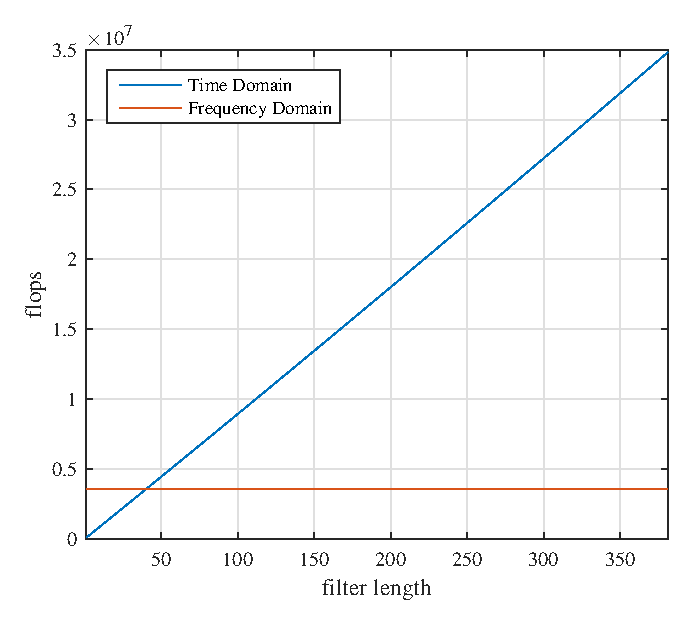
\includegraphics[width=5in]{figures/gpu_intro/Theory12672signal_flops.eps}
	\label{fig:Theory12672signal_flops}
	\caption{Comparison of number of floating point operations (flops) required to convolve a $12672$ sample complex signal with a varied length tap complex filter.}
\end{figure}

Figure \ref{fig:Theory186Tap_flops} compares the number of flops required for time-domain verse frequency-domain convolution of a $12672$ sample complex signal with a $186$ tap complex filter.
Figure \ref{fig:Theory21Tap_flops} compares the number of flops required for time-domain verse frequency-domain convolution of a $12672$ sample complex signal with a $21$ tap complex filter.
Appending zeros to the next power of $2$ causes the stair stepping pattern.
Judging by the figures with varied signal lengths, a $186$ tap filter is ``long'' and a $21$ tap filter is ``short.''
\begin{figure}
	\centering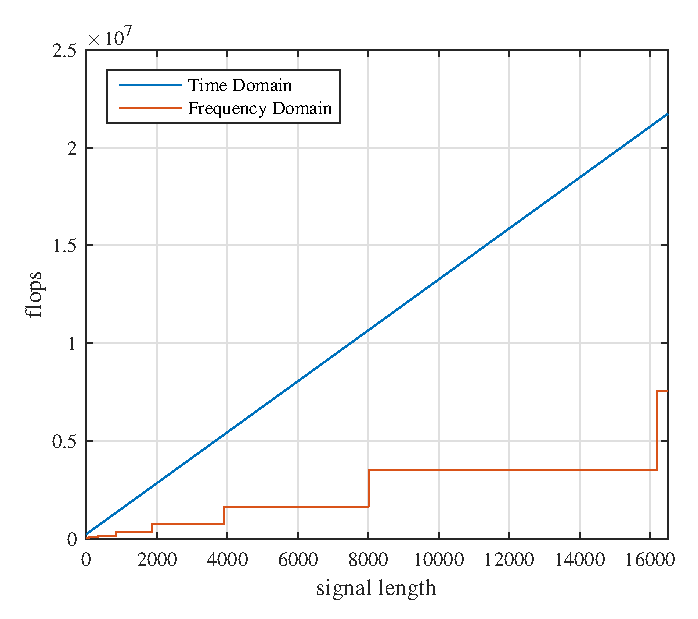
\includegraphics[width=5in]{figures/gpu_intro/Theory186Tap_flops.eps}
	\label{fig:Theory186Tap_flops}
	\caption{Comparison of number of floating point operations (flops) required to convolve a varied length complex signal with a $186$ tap complex filter.}
\end{figure}
\begin{figure}
	\centering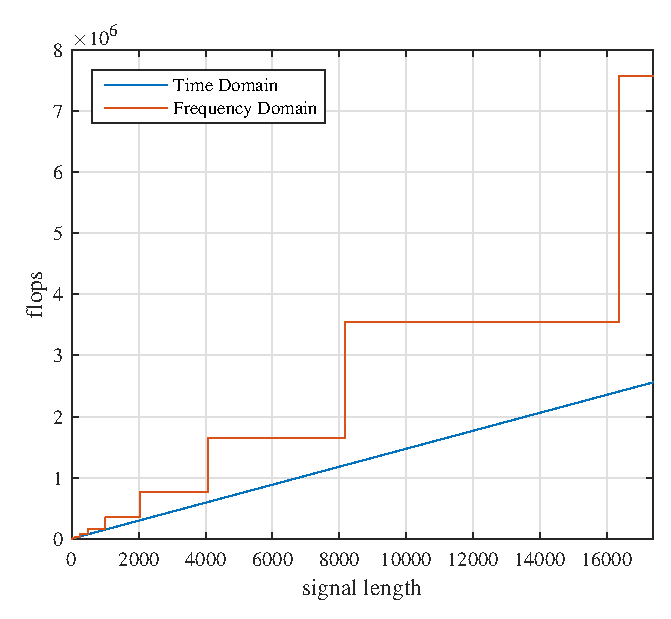
\includegraphics[width=5in]{figures/gpu_intro/Theory21Tap_flops.eps}
	\label{fig:Theory21Tap_flops}
	\caption{Comparison of number of floating point operations (flops) required to convolve a varied length complex signal with a $21$ tap complex filter.}
\end{figure}



\section{CPU and GPU Single Batch Convolution}
\label{sec:cuda_convolution_single}
With an understanding of the number of flops in time verses frequency domain required to implement convolution,
do the number of flops have a direct relationship to execution time in CPUs and GPUS?
To explore the flop to execution time relationship Listing \ref{code:convFun} shows five different ways of implementing convolution:
\begin{itemize}
  \item time-domain convolution in a CPU
  \item frequency-domain convolution in a CPU
  \item time-domain convolution in a GPU using global memory
  \item time-domain convolution in a GPU using shared memory
  \item frequency-domain convolution in a GPU using CUDA libraries
\end{itemize}

The CPU implements Equation \eqref{eq:simple_conv_time} in ConvCPU directly on line $209$ using a function from lines $11$ to $34$.
The CPU implements Equation \eqref{eq:simple_conv_freq} using the FFTW library on lines $214$ to $258$.

The GPU implements time-domain convolution using global memory in lines $268$ to $277$.
The GPU kernel ConvGPU on lines $36$ to $64$ is a parallel version of ConvCPU.
ConvGPU performs time-domain convolution by fetching every element of the signal and filter from global memory.

The GPU implements time-domain convolution using shared memory in lines $283$ to $292$.
The GPU kernel ConvGPUshared on lines $67$ to $101$ is nearly identical to ConvGPU.
Threads accessing the same elements of the filter in global memory can be a waste of valuable clock cycles.
ConvGPUshared pays and initial price on lines $72$ to $76$ to move $L_\text{h}$ filter coefficients from off chip global memory to the on chip shared memory.
Finally, the GPU implements frequency-domain convolution using the cuFFT library on lines $298$ to $326$.

The questions are:
Do flops have a direct relationship to execution time on CPUs? 
Do flops have a direct relationship to execution time on GPUs? 
When is the initial cost to use shared memory worth it?
When should convolution be done in the frequency domain?

The short answer to all of the questions is: GPU execution time depend on the signal length, filter length, CPU, GPU and memory.
A good CUDA programmer can make an educated guess on which algorithm may be faster in the GPU, but until all the algorithms have been implemented and timed, there is no definite answer.

To demonstrate that there is no definite answer in GPUs, 
the execution time of the code in Listing \ref{code:GPUvsCPU} was timed.
All the memory transfers to and from the host were timed for a fair comparison of GPU to CPU.
Table \ref{tab:CPUvsGPUtimingTable} shows where timing was started and stopped for each convolution implementation.
\begin{table}
\caption{Defining start and stop lines for timing comparison in Listing \ref{code:convFun}.}
\begin{center}
\begin{tabular}{llll}
	\toprule
	Algorithm 				& Function		& Start Line	& Stop  Line		\\ \midrule
	CPU time domain 		& ConvCPU 		& 208			& 210 				\\
	CPU frequency domain 	& FFTW 			& 213			& 259 				\\
	GPU time domain global 	& ConvGPU 		& 267			& 278				\\
	GPU time domain shared 	& ConvGPUshared & 282			& 293				\\
	GPU frequency domain 	& cuFFT			& 301			& 327				\\ 
	\bottomrule
\end{tabular}
\end{center}
\label{tab:CPUvsGPUtimingTable}
\end{table}

The execution times shown in Figure \ref{fig:CPUvsGPU_1batch_186taps_varySignal_noMin} compares the computation time of a fixed length $186$ tap filter convolved with a varied length signal.
The CPU execution time varies enough that the plot is messy.
Figure \ref{fig:CPUvsGPU_1batch_186taps_varySignal} shows the lower bounds of execution times by finding the local minimums in $15$ sample windows.
\begin{figure}
	\centering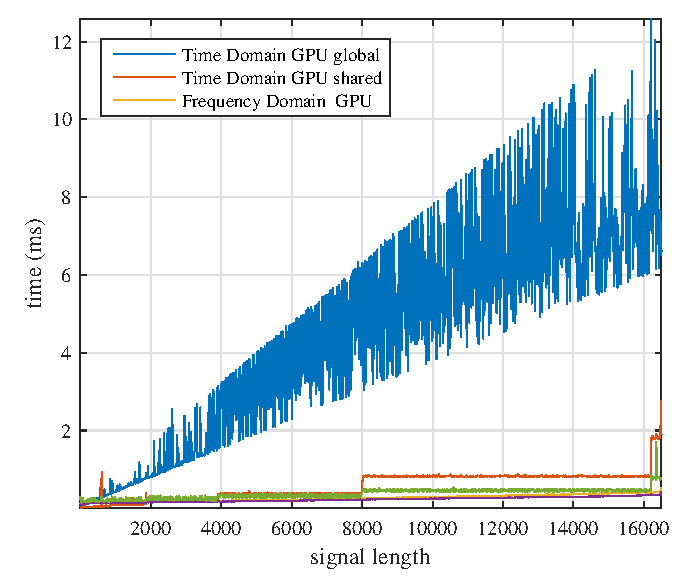
\includegraphics[width=5in]{figures/gpu_intro/CPUvsGPU_1batch_186taps_varySignal_noMin.eps}
	\label{fig:CPUvsGPU_1batch_186taps_varySignal_noMin}
	\caption{Comparison of a complex convolution on CPU verse GPU. The signal length is varied and the filter is fixed at $186$ taps. The comparison is messy with out lower bounding.}
\end{figure}
\begin{figure}
	\centering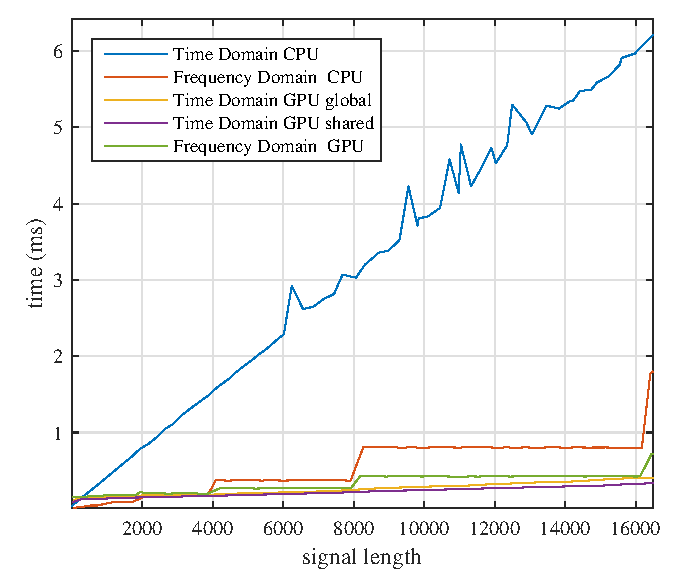
\includegraphics[width=5in]{figures/gpu_intro/CPUvsGPU_1batch_186taps_varySignal.eps}
	\label{fig:CPUvsGPU_1batch_186taps_varySignal}
	\caption{Comparison of a complex convolution on CPU verse GPU. The signal length is varied and the filter is fixed at $186$ taps. A lower bound was applied by searching for a local minimums in $15$ sample width windows.}
\end{figure}

With the plot lower bounded, compare Figure \ref{fig:CPUvsGPU_1batch_186taps_varySignal} to Figure \ref{fig:Theory186Tap_flops}.
Does the CPU and GPU follow the same trend as the number of flops?
The CPU has the exact structure that the number of flops predicted.
The GPU does have the stair stepping from appending zeros for the frequency domain, but the time domain GPU kernels perform better than the number of flops predicted.

The GPU execution time does not follow the same trend as the number of flops.
Why? As mentioned in Section \ref{sec:GPU_memory}, GPUs have a ridiculous amount of computational resources and limited memory bandwidth.
Over $90\%$ of GPU kernels are memory bandwidth limited.
Fast GPU kernels access memory efficiently.

To provide more proof, compare Figures \ref{fig:CPUvsGPU_1batch_21taps_varySignal} and \ref{fig:Theory21Tap_flops}.
Once again, the CPU follows the same trend as the number of flops.
The GPU also follows the number of flops trends but to a lesser extent than the CPU.
Using shared memory will perform better than using only global memory for ``short'' filters.
\begin{figure}
	\centering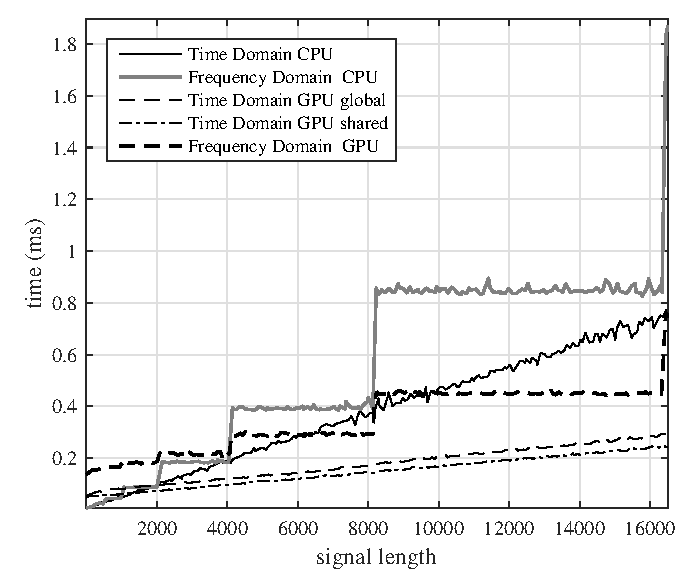
\includegraphics[width=5in]{figures/gpu_intro/CPUvsGPU_1batch_21taps_varySignal.eps}
	\label{fig:CPUvsGPU_1batch_21taps_varySignal}
	\caption{Comparison of a complex convolution on CPU verse GPU. The signal length is varied and the filter is fixed at $21$ taps. A lower bound was applied by searching for a local minimums in $5$ sample width windows.}
\end{figure}

What if the signal length was set and the filter length was varied?
Comparing Figure \ref{fig:CPUvsGPU_1batch_12672signal_varyFilter} to Figure \ref{fig:Theory12672signal_flops} shows the CPU follows the trend of flops also.
The time domain CPU execution time is obviously affected as the number of flops increases.
Neither CPU or GPU frequency domain execution time is affected by varying filter length.

The execution time of both time-domain GPU convolutions are slightly affected by increasing filter length.
The number of memory accesses per output sample increase as the filter length increases.
Bottom line, the length of the signal is the largest factor as Equations \ref{eq:flops_time_domain_conv} and \ref{eq:flops_freq_domain_conv} suggest.
\begin{figure}
	\centering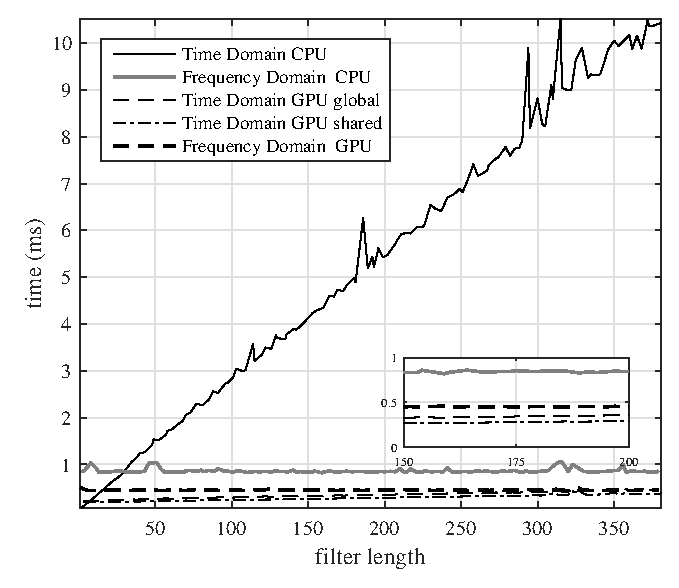
\includegraphics[width=5in]{figures/gpu_intro/CPUvsGPU_1batch_12672signal_varyFilter.eps}
	\label{fig:CPUvsGPU_1batch_12672signal_varyFilter}
	\caption{Comparison of a complex convolution on CPU verse GPU. The filter length is varied and the signal is fixed at $12672$ samples. A lower bound was applied by searching for a local minimums in $3$ sample width windows.}
\end{figure}

For most convolution implementations, the signal and filter lengths are set ``magic'' numbers.
To find the best option, implement convolution every way possible for the given lengths, time each implementation execution time, choose which algorithm is fastest.
As Figures \ref{fig:CPUvsGPU_1batch_186taps_varySignal_noMin} through \ref{fig:CPUvsGPU_1batch_12672signal_varyFilter} have shown, unless every implementation is explored, there is no way of saying which implementation will absolutely be fastest.

Table \ref{tab:CPUvsGPUtable_12672_186} shows the GPU frequency-domain algorithm is fastest when convolving a $12672$ sample signal with a $186$ tap filter.
Table \ref{tab:CPUvsGPUtable_12672_21} shows the GPU time-domain algorithm using shared memory is fastest when convolving a $12672$ sample signal with a $21$ tap filter.
\begin{table}
\caption{Convolution computation times with signal length $12672$ and filter length $186$ on a Tesla K40c GPU.}
\begin{center}
\begin{tabular}{lll}
	\toprule
	Algorithm 				& Function or Library		& Execution Time (ms) \\ \midrule
	CPU time domain 		& ConvCPU 					& 5.3000		\\
	CPU frequency domain 	& FFTW 						& 0.7972		\\
	GPU time domain global 	& ConvGPU 					& 0.3321		\\
	GPU time domain shared 	& ConvGPUshared 			& 0.2748		\\
	GPU frequency domain 	& cuFFT						& 0.4224		\\ 
	\bottomrule
\end{tabular}
\end{center}
\label{tab:CPUvsGPUtable_12672_186}
\end{table}
\begin{table}
\caption{Convolution computation times with signal length $12672$ and filter length $21$ on a Tesla K40c GPU.}
\begin{center}
\begin{tabular}{lll}
	\toprule
	Algorithm 				& Function or Library		& Execution Time (ms) \\ \midrule
	CPU time domain 		& ConvCPU 					& 0.5878		\\
	CPU frequency domain 	& FFTW 						& 0.8417		\\
	GPU time domain global 	& ConvGPU 					& 0.4476		\\
	GPU time domain shared 	& ConvGPUshared 			& 0.1971		\\
	GPU frequency domain 	& cuFFT						& 0.3360		\\ 
	\bottomrule
\end{tabular}
\end{center}
\label{tab:CPUvsGPUtable_12672_21}
\end{table}

\section{Batched Convolution}
As shown in section \ref{sec:cuda_convolution_single}, single convolution doesn't leverage the full power of parallel processing in GPUs.
The introduction showed the PAQ project received signal has a packetized structure.
The received signal has $3104$ packets or batches.
Batched processing introduces an extra level of parallelism in GPUs because each batch can be processed independently.
CUDA has many libraries that are ``batched,'' meaning a GPU kernel is launched for each independent packet or batch of received samples.
Some CUDA batched libraries used in PAQ system are cuFFT, cuBLAS and cuSolver.
%Figure \ref{fig:matrix_batch_vs_batched} shows the concept of a batched matrix multiply.
%\begin{figure}
%	\centering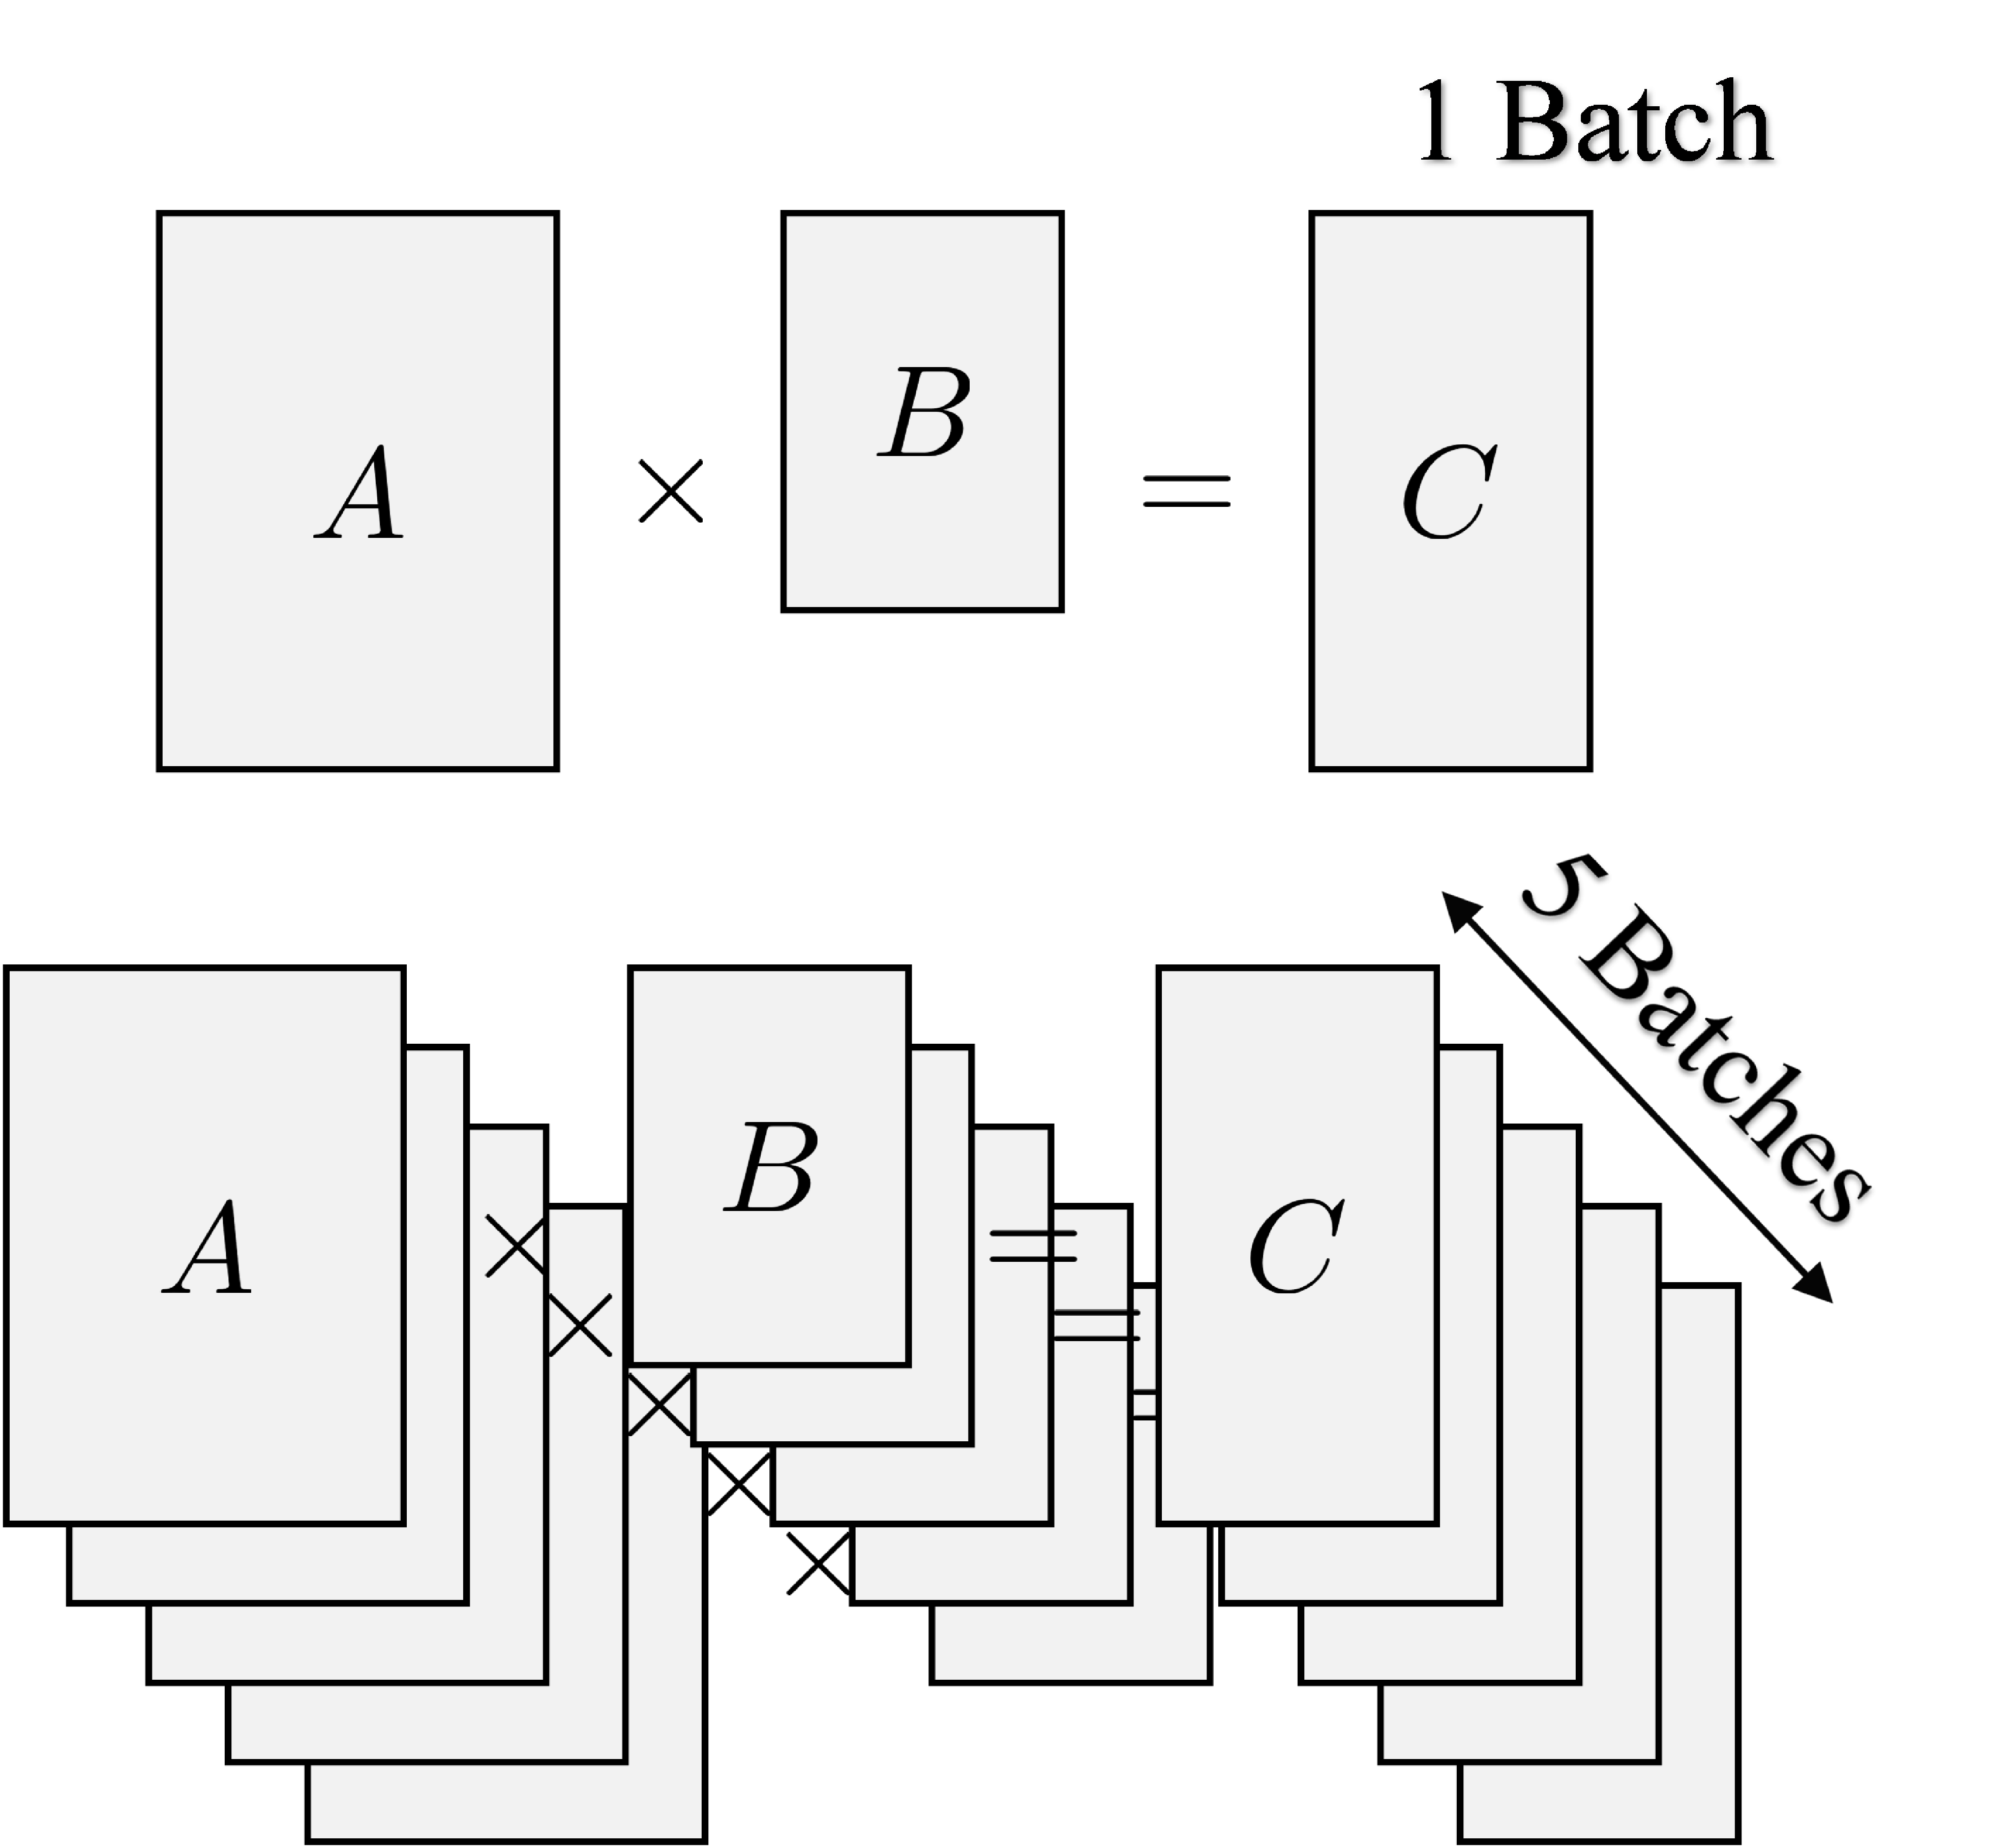
\includegraphics[width=4.13in/100*55]{figures/eq_GPUimplementation/matrix_batch_vs_batched.pdf}
%	\label{fig:matrix_batch_vs_batched}
%	\caption{Diagram showing the relationships between $z(n)$, $\rho(n)$ and $b(n)$.}
%\end{figure}

Batched libraries perform much better than calling a single GPU kernel multiple times with each independent batch of data.
Haidar et al. showed batched libaries in GPUs achive more Gflops than calling GPU kernels multiple times \cite{haidar2015optimization}.
Batched processing performs very well in GPUs because it increases parallelism, reduces overhead on the CPU and provides more opportunities for NVIDIA engineers to optimize.

As the number of batches increases, does CPU and GPU execution time increase linearly?
To illistrate how batch processing performs on GPUs, Figure \ref{fig:CPUvsGPU_varyBatches_186taps_12672signal_timePerBatch} shows the execution time per batch for batched convolution in GPUs.
The execution time per batch decreases as the number of batches increases but converges after $70$ batches.
\begin{figure}
	\centering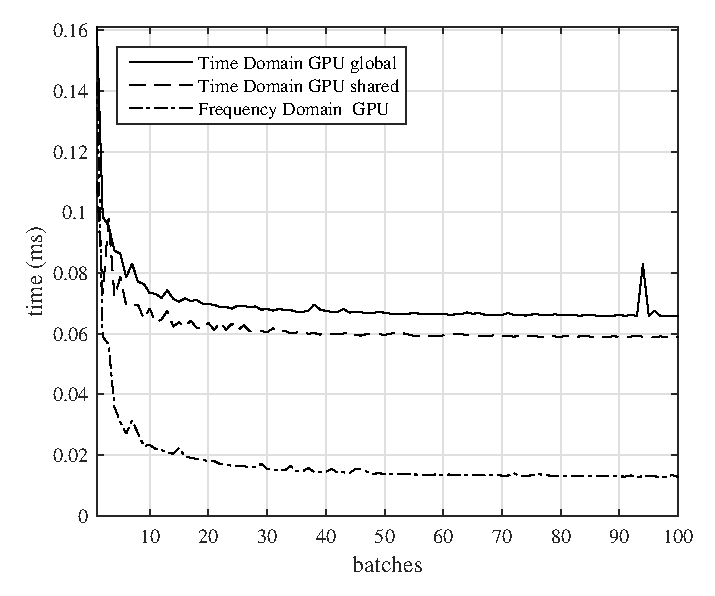
\includegraphics[width=5in]{figures/gpu_intro/CPUvsGPU_varyBatches_186taps_12672signal_timePerBatch.eps}
	\label{fig:CPUvsGPU_varyBatches_186taps_12672signal_timePerBatch}
	\caption{Comparison on execution time per batch for complex convolution. The number of batches is varied while the signal and filter length is set to $12672$ and $186$.}
\end{figure}

Figure \ref{fig:CPUvsGPU_varyBatches_186taps_12672signal} shows how the execution time increases with the number of batches varied.
Note that no lower bounding is needed to produce clean batched processing results.
This figure shows that frequency-domain convolution leverages batch processing better than time-domain convolution.
No surprise CPU time and frequency domain execution time skyrockets as the number of batches increases.
\begin{figure}
	\centering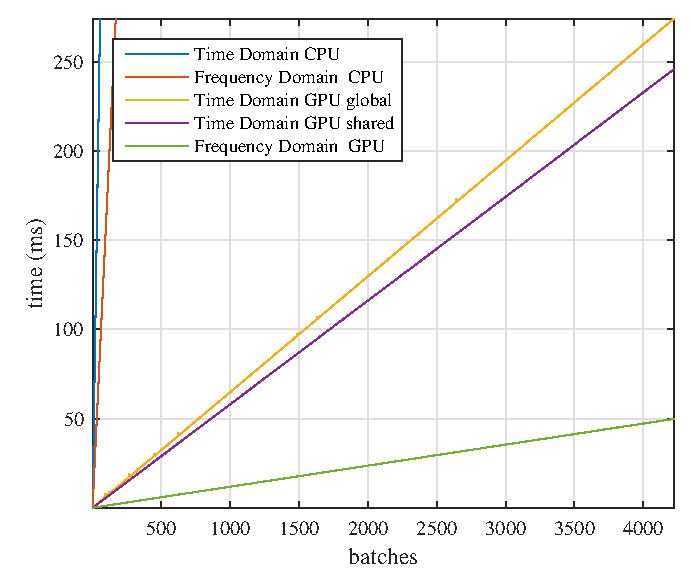
\includegraphics[width=5in]{figures/gpu_intro/CPUvsGPU_varyBatches_186taps_12672signal.eps}
	\label{fig:CPUvsGPU_varyBatches_186taps_12672signal}
	\caption{Comparison of a batched complex convolution on a CPU and GPU. The number of batches is varied while the signal and filter length is set to $12672$ and $186$.}
\end{figure}

Judging by Figure \ref{fig:CPUvsGPU_varyBatches_186taps_12672signal}, CPU is not a contender in batched processing compared to the GPU.
CPU batched processing will not be explored any further.
Listing \ref{code:batchedConvFun} shows three implementations of batched convolution in CUDA
\begin{itemize}
  \item time-domain convolution in a GPU using global memory
  \item time-domain convolution in a GPU using shared memory
  \item frequency-domain convolution in a GPU using the cuFFT library.
\end{itemize}

Now that the GPU execution time isn't being compared to the CPU, transfers between host and device will not be a factor for algorithm comparison.
Table \ref{tab:BatchedGPUtimingTable} shows how Listing \ref{code:batchedConvFun} is timed.
\begin{table}
\caption{Defining start and stop lines for timing comparison in Listing \ref{code:batchedConvFun}.}
\begin{center}
\begin{tabular}{llll}
	\toprule
	Algorithm 				& Function		& Start Line	& Stop  Line		\\ \midrule
	GPU time domain global 	& ConvGPU 		& 197			& 204				\\
	GPU time domain shared 	& ConvGPUshared & 212			& 219				\\
	GPU frequency domain 	& cuFFT			& 227			& 245				\\ 
	\bottomrule
\end{tabular}
\end{center}
\label{tab:BatchedGPUtimingTable}
\end{table}
Figure \ref{fig:CPUvsGPU_3104batch_186taps_varySignal} shows execution time for $3104$ batches of $186$ tap filters convolved with varying signal lengths.
Performing frequency-domain convolution is always faster than time-domain convolution because the cuFFT library is better optimized for batched processing.
The batched GPU implementation of convolution in the frequency-domain convolution takes just $36.8$ms for $3104$ batches, $12672$ sample signals and $186$ tap filters.
The average exectution time per batch for $3104$ batches is $0.0119$ms per batch!
Compare $0.0119$ms per batch to single batched execution time in Table \ref{tab:CPUvsGPUtable_12672_186}, one batch took $0.4224$.
Batched processing introduced a $35\times$ speed up!
\begin{figure}
	\centering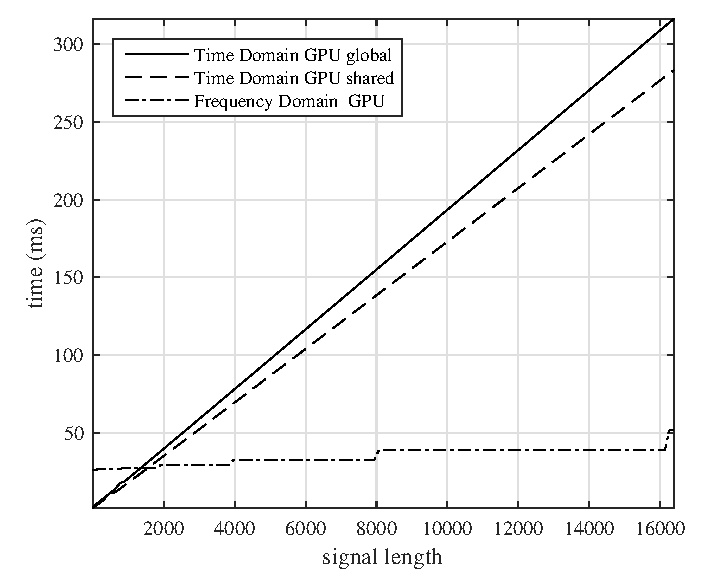
\includegraphics[width=5in]{figures/gpu_intro/CPUvsGPU_3104batch_186taps_varySignal.eps}
	\label{fig:CPUvsGPU_3104batch_186taps_varySignal}
	\caption{Comparison of a batched complex convolution on a GPU. The signal length is varied and the filter is fixed at $186$ taps.}
\end{figure}

Figure \ref{fig:CPUvsGPU_3104batch_21taps_varySignal} shows execution time for $3104$ batches of $21$ tap filters convolved with varying signal lengths.
This figure exhibits the same characteristics of single batch convolution execution time shown in Figure \ref{fig:CPUvsGPU_1batch_21taps_varySignal}.
For most signal lengths, performing time-domain convolution using shared memory is fastest.
\begin{figure}
	\centering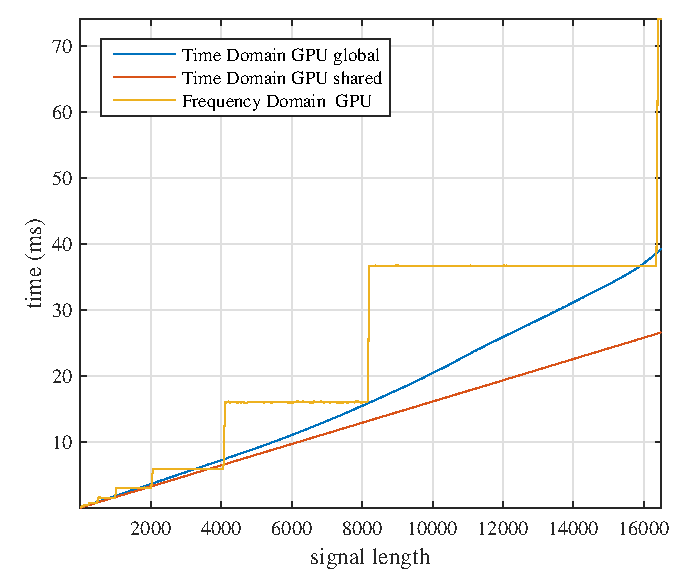
\includegraphics[width=5in]{figures/gpu_intro/CPUvsGPU_3104batch_21taps_varySignal.eps}
	\label{fig:CPUvsGPU_3104batch_21taps_varySignal}
	\caption{Comparison of a batched complex convolution on a GPU. The signal length is varied and the filter is fixed at $21$ taps.}
\end{figure}

Figure \ref{fig:CPUvsGPU_3104batch_12672signal_varyFilter} shows execution time for $3104$ batches of $12672$ sample signal convolved with varying filter lengths.
This figure exhibits nearly the same characteristics of single batch convolution execution time shown in Figure \ref{fig:CPUvsGPU_1batch_12672signal_varyFilter} accept the varied filter length has no affect on execution time.
For very short filter lengths, time-domain convolution using shared memory is fastest.
For longer filters , frequency-domain convolution is fastest.
\begin{figure}
	\centering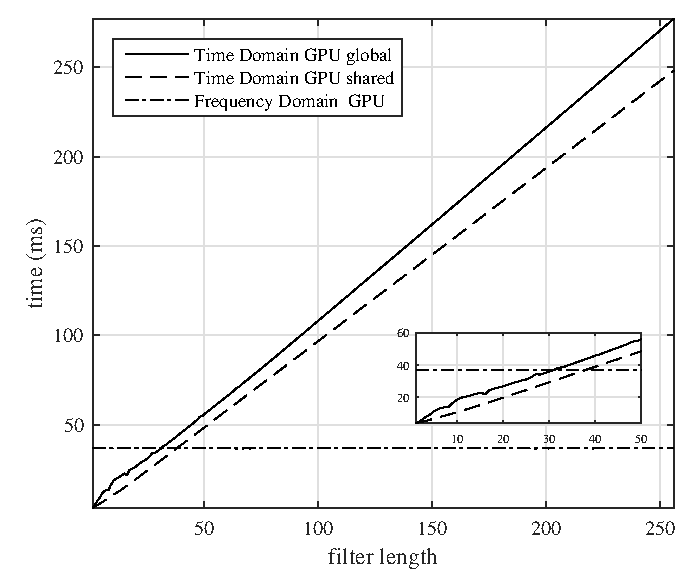
\includegraphics[width=5in]{figures/gpu_intro/CPUvsGPU_3104batch_12672signal_varyFilter.eps}
	\label{fig:CPUvsGPU_3104batch_12672signal_varyFilter}
	\caption{Comparison of a batched complex convolution on a GPU. The filter length is varied and the signal length is set at $12672$ samples.}
\end{figure}

Though this section has show the power of batched processing, the algorithm leading to the fastest execution time still depends on signal and filter length,
One important concept has been over looked.
Figure \ref{fig:thisThesisBlock} shows there are two filters that need to be applied to the received samples. 

If convolution is implemented in the time domain, ConvGPU or ConvGPUshared must run twice.
The first call of time-domain convolution performs an extremely fast ``short'' convolution of the $186$ tap equalizer and $21$ detection filter.
The second call performs a slower ``long'' convolution of the $12672$ sample signal with the  convolved $186+21-1$ tap filter.

If convolution is implemented in the frequency domain, only the GPU kernel PointToPointMultiply has to be updated.
PointToPointMultiply is changed from two to three input vectors.
For every point the number of memory accesses increases by $1$ element and the number of flops doubles from $6$ to $12$.
An extra cuFFT call would be expected accept the detection filter is predefined in Figure \ref{fig:thisThesisBlock}.
The FFT of the detection filter is calculated and stored at initialization.

Table \ref{tab:Batched_CPUvsGPUtable_12672_186} shows the batched convolution execution time for a $12672$ sample signal and $186$ tap filter.
Table \ref{tab:Batched_CPUvsGPUtable_12672_21} shows the batched convolution execution time for a $12672$ sample signal and $21$ tap filter.
Table \ref{tab:Batched_CPUvsGPUtable_12672_21_186} shows batched cascaded $21$ and $186$ tap filters convolved with a $12672$ sample signal execution time.
\begin{table}
\caption{Batched convolution execution times with for a $12672$ sample signal and $186$ tap filter on a Tesla K40c GPU.}
\begin{center}
\begin{tabular}{lll}
	\toprule
	Algorithm 				& Function or Library		& Execution Time (ms) \\ \midrule
	GPU time domain global 	& ConvGPU 					& 201.29		\\
	GPU time domain shared 	& ConvGPUshared 			& 180.272		\\
	GPU frequency domain 	& cuFFT						& 36.798 		\\ 
	\bottomrule
\end{tabular}
\end{center}
\label{tab:Batched_CPUvsGPUtable_12672_186}
\end{table}
\begin{table}
\caption{Batched convolution execution times with for a $12672$ sample signal and $21$ tap filter on a Tesla K40c GPU.}
\begin{center}
\begin{tabular}{lll}
	\toprule
	Algorithm 				& Function or Library		& Execution Time (ms) \\ \midrule
	GPU time domain global 	& ConvGPU 					& 27.642		\\
	GPU time domain shared 	& ConvGPUshared 			& 20.4287		\\
	GPU frequency domain 	& cuFFT						& 36.7604		\\ 
	\bottomrule
\end{tabular}
\end{center}
\label{tab:Batched_CPUvsGPUtable_12672_21}
\end{table}
\begin{table}
\caption{Batched convolution execution times with for a $12672$ sample signal and cascaded $21$ and $186$ tap filter on a Tesla K40c GPU.}
\begin{center}
\begin{tabular}{lll}
	\toprule
	Algorithm 				& Function or Library		& Execution Time (ms) \\ \midrule
	GPU time domain global 	& ConvGPU 					& 223.307		\\
	GPU time domain shared 	& ConvGPUshared 			& 200.018		\\
	GPU frequency domain 	& cuFFT						& 39.0769		\\ 
	\bottomrule
\end{tabular}
\end{center}
\label{tab:Batched_CPUvsGPUtable_12672_21_186}
\end{table}
\begin{table}
\caption{Batched convolution execution times with for a $12672$ sample signal and $206$ tap filter on a Tesla K40c GPU.}
\begin{center}
\begin{tabular}{lll}
	\toprule
	Algorithm 				& Function or Library		& Execution Time (ms) \\ \midrule
	GPU time domain global 	& ConvGPU 					& 223.064		\\
	GPU time domain shared 	& ConvGPUshared 			& 199.844		\\
	GPU frequency domain 	& cuFFT						& 36.7704		\\ 
	\bottomrule
\end{tabular}
\end{center}
\label{tab:Batched_CPUvsGPUtable_12672_206}
\end{table}

Tables \ref{tab:Batched_CPUvsGPUtable_12672_186} and \ref{tab:Batched_CPUvsGPUtable_12672_21} agree with Figures \ref{fig:CPUvsGPU_3104batch_21taps_varySignal} and \ref{fig:CPUvsGPU_3104batch_186taps_varySignal}.
time-domain convolution is faster with a short $21$ tap filter but frequency-domain convolution is faster with a long $186$ tap filter.

\begin{figure}
	\centering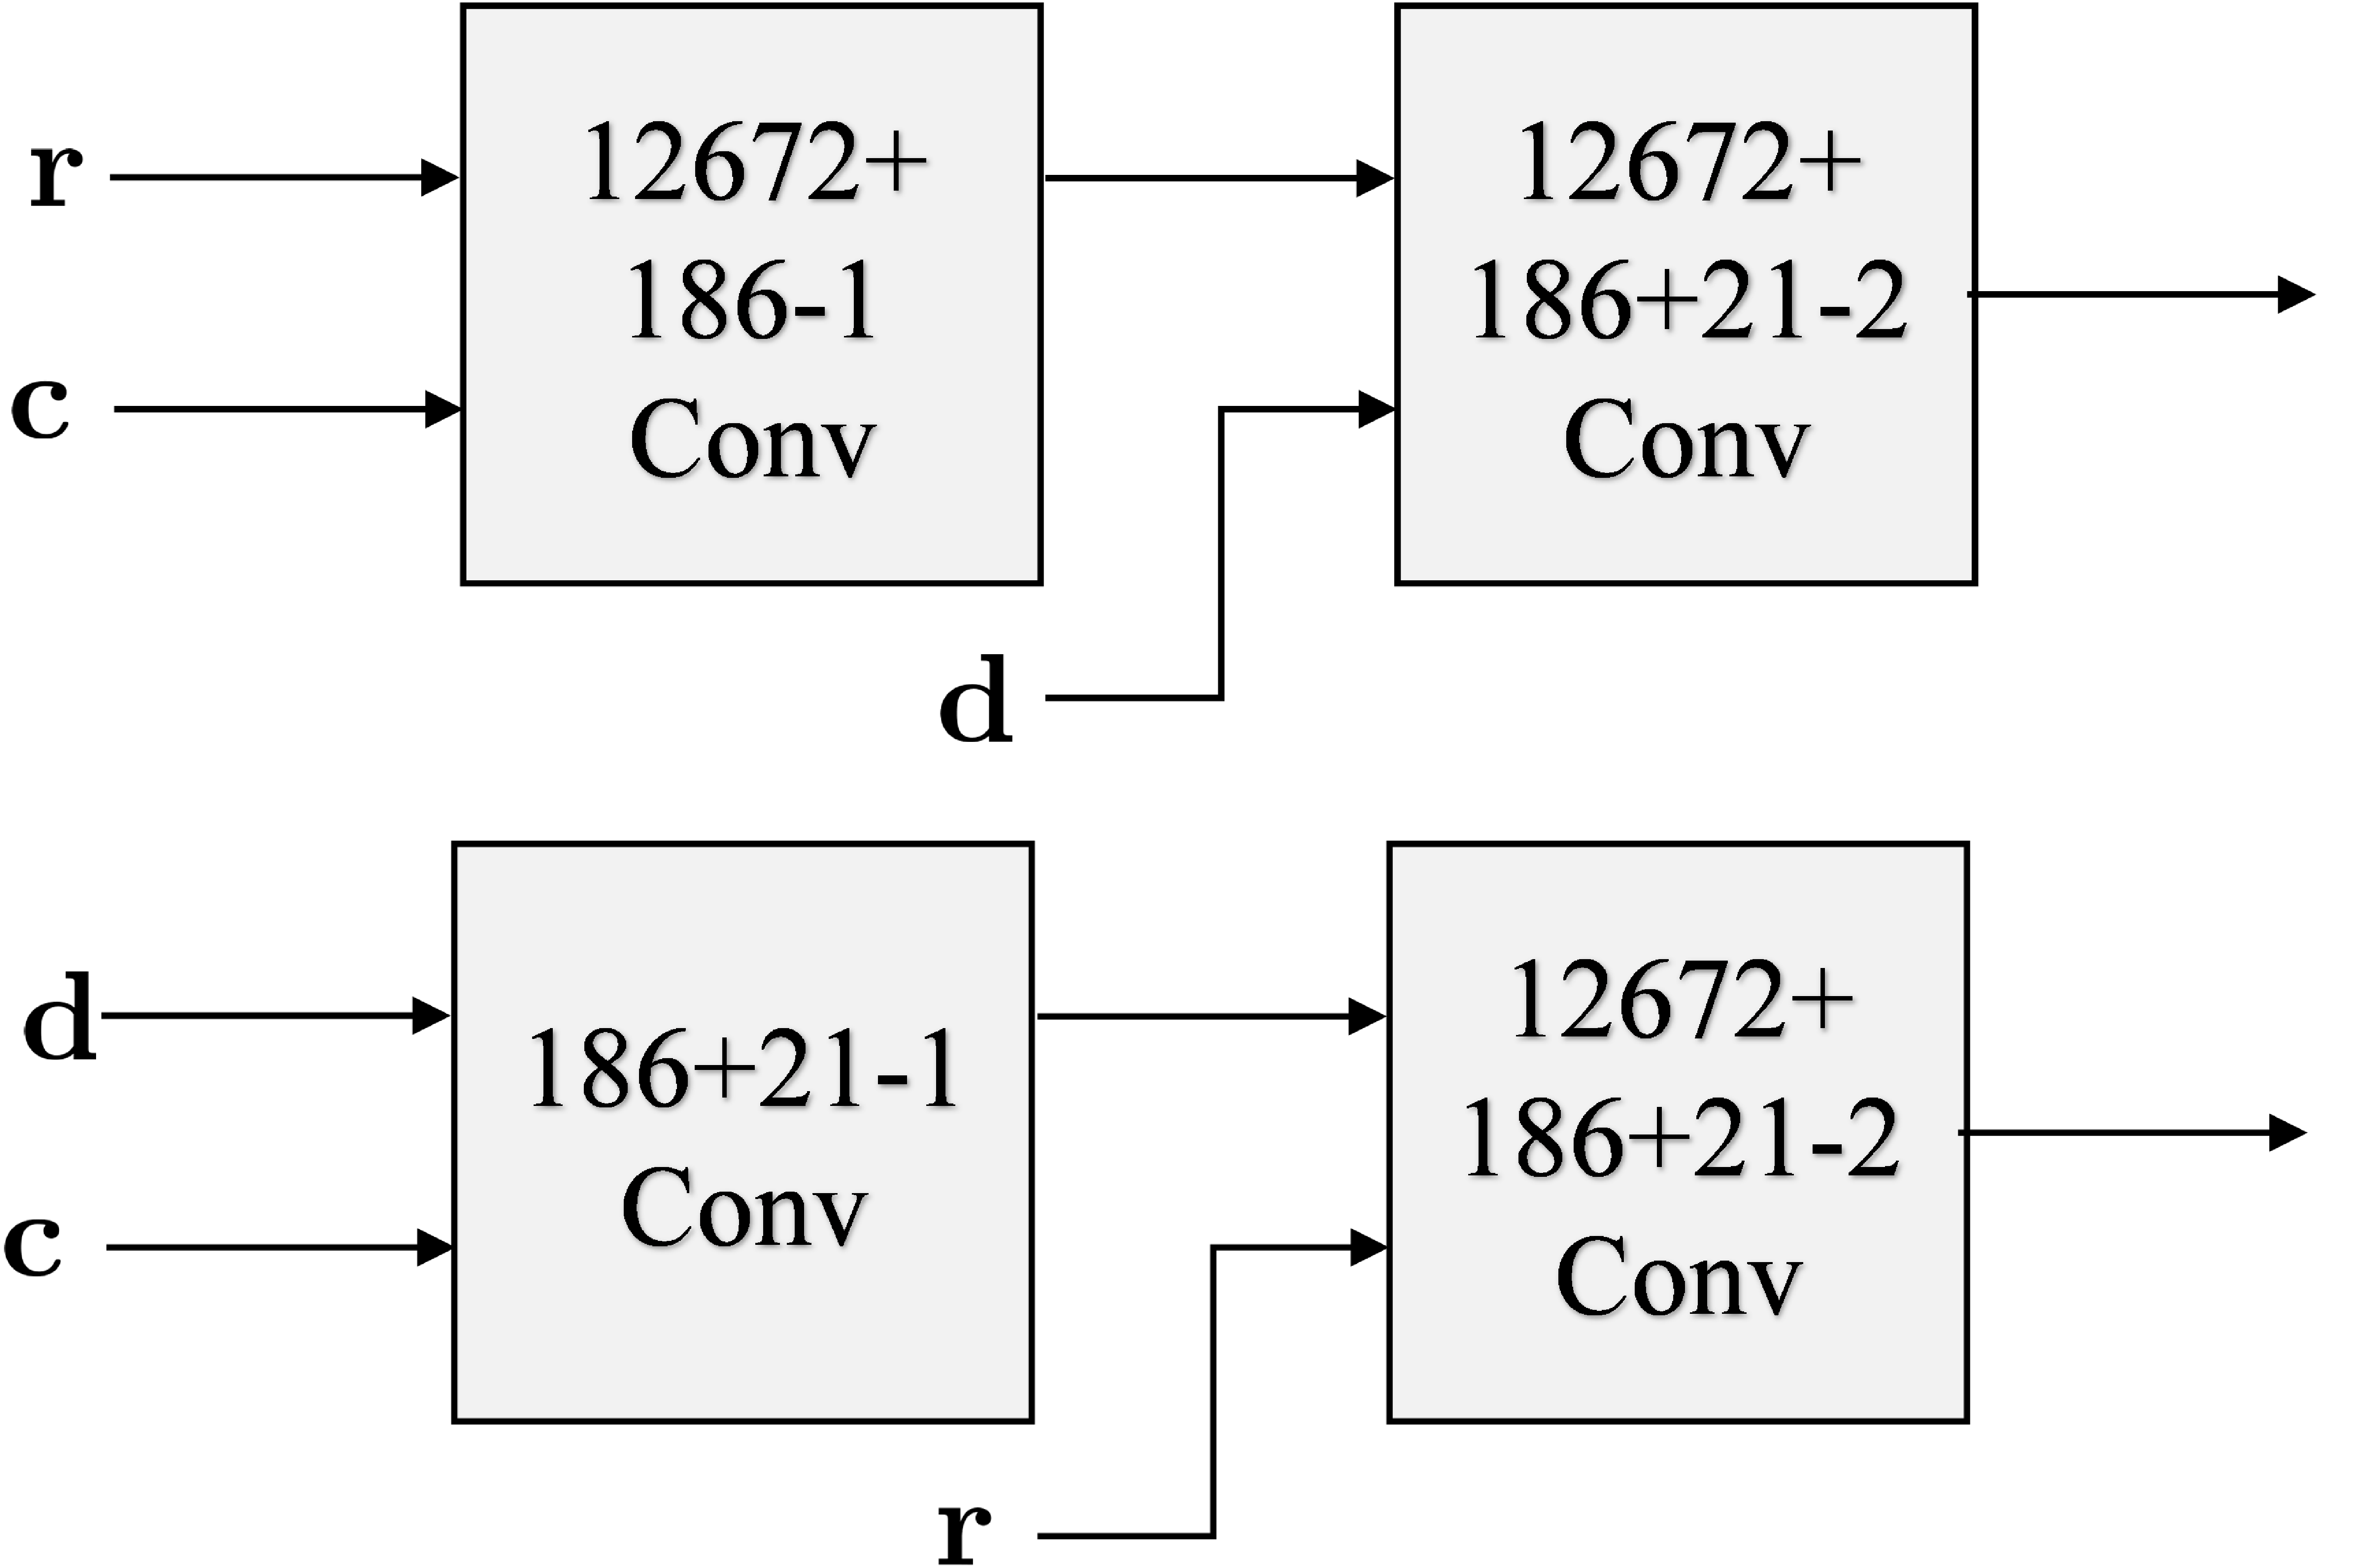
\includegraphics[width=5.01in/100*55]{figures/gpu_intro/twoWaysToConv.pdf}
	\label{fig:twoWaysToConv}
	\caption{Two ways to convolve the signal $\mathbf{r}$ with the $186$ tap filter $\mathbf{c}$ and $21$ tap filter $\mathbf{d}$.}
\end{figure}
Figure \ref{fig:twoWaysToConv} shows two ways to cascade the signal $\mathbf{r}$ though two filters.
The upper blocks apply both filters to the signal taking $180.272$ms then $20.4287$ms.
The lower blocks first convolve the filters to build a $186+21-1$ tap composite filter then apply the $206$ tap composite to the signal.

Table \ref{tab:Batched_CPUvsGPUtable_12672_21_186} shows the execution time of implementing cascaded filters, convolving the $21$ and $186$ tap filters is extremely fast in the GPU.
While building the composite filter is extremely fast, time-domain convolution suffers a $22.0170$ms or $19.7460$ms slow down because the composite filter is now $206$ taps.
Applying an extra filter in the frequency domain only costs $2.3165$ms.
Table \ref{tab:Batched_CPUvsGPUtable_12672_206} confirms it costs an extra $20$ms or so to apply a $206$ vs $186$ tap filter.

\singlespacing
\clearpage
\begin{lstlisting}[style=myCUDAstyle,language=C++,caption={CUDA code to performing complex convolution five different ways: time domain CPU, frequency domain CPU time domain GPU, time domain GPU using shared memory and frequency domain GPU.},label={code:convFun}]
#include <iostream>
#include <stdlib.h>
#include <math.h>
#include <cufft.h>
#include <fstream>
#include <string>
#include <fftw3.h>
using namespace std;


void ConvCPU(cufftComplex* y,cufftComplex* x,cufftComplex* h,int Lx,int Lh){
	for(int yIdx = 0; yIdx < Lx+Lh-1; yIdx++){
		cufftComplex temp;
		temp.x = 0;
		temp.y = 0;
		for(int hIdx = 0; hIdx < Lh; hIdx++){
			int xAccessIdx = yIdx-hIdx;
			if(xAccessIdx>=0 && xAccessIdx<Lx){
				// temp += x[xAccessIdx]*h[hIdx];
				float A = x[xAccessIdx].x;
				float B = x[xAccessIdx].y;
				float C = h[hIdx].x;
				float D = h[hIdx].y;
				cufftComplex result;
				result.x = A*C-B*D;
				result.y = A*D+B*C;
				temp.x += result.x;
				temp.y += result.y;
			}
		}
		y[yIdx] = temp;
	}

}

__global__ void ConvGPU(cufftComplex* y,cufftComplex* x,cufftComplex* h,int Lx,int Lh){
	int yIdx = blockIdx.x*blockDim.x + threadIdx.x;

	int lastThread = Lx+Lh-1;

	// don't access elements out of bounds
	if(yIdx >= lastThread)
		return;

	cufftComplex temp;
	temp.x = 0;
	temp.y = 0;
	for(int hIdx = 0; hIdx < Lh; hIdx++){
		int xAccessIdx = yIdx-hIdx;
		if(xAccessIdx>=0 && xAccessIdx<Lx){
			// temp += x[xAccessIdx]*h[hIdx];
			float A = x[xAccessIdx].x;
			float B = x[xAccessIdx].y;
			float C = h[hIdx].x;
			float D = h[hIdx].y;
			cufftComplex result;
			result.x = A*C-B*D;
			result.y = A*D+B*C;
			temp.x += result.x;
			temp.y += result.y;
		}
	}
	y[yIdx] = temp;
}


__global__ void ConvGPUshared(cufftComplex* y,cufftComplex* x,cufftComplex* h,int Lx,int Lh){
	int yIdx = blockIdx.x*blockDim.x + threadIdx.x;

	int lastThread = Lx+Lh-1;

	extern __shared__ cufftComplex h_shared[];
	if(threadIdx.x < Lh){
		h_shared[threadIdx.x] = h[threadIdx.x];
	}
	__syncthreads();

	// don't access elements out of bounds
	if(yIdx >= lastThread)
		return;

	cufftComplex temp;
	temp.x = 0;
	temp.y = 0;
	for(int hIdx = 0; hIdx < Lh; hIdx++){
		int xAccessIdx = yIdx-hIdx;
		if(xAccessIdx>=0 && xAccessIdx<Lx){
			// temp += x[xAccessIdx]*h[hIdx];
			float A = x[xAccessIdx].x;
			float B = x[xAccessIdx].y;
			float C = h_shared[hIdx].x;
			float D = h_shared[hIdx].y;
			cufftComplex result;
			result.x = A*C-B*D;
			result.y = A*D+B*C;
			temp.x += result.x;
			temp.y += result.y;
		}
	}
	y[yIdx] = temp;
}

__global__ void PointToPointMultiply(cufftComplex* v0, cufftComplex* v1, int lastThread){
	int i = blockIdx.x*blockDim.x + threadIdx.x;

	// don't access elements out of bounds
	if(i >= lastThread)
		return;
	float A = v0[i].x;
	float B = v0[i].y;
	float C = v1[i].x;
	float D = v1[i].y;

	// (A+jB)(C+jD) = (AC-BD) + j(AD+BC)
	cufftComplex result;
	result.x = A*C-B*D;
	result.y = A*D+B*C;

	v0[i] = result;
}

__global__ void ScalarMultiply(cufftComplex* vec0, float scalar, int lastThread){
	int i = blockIdx.x*blockDim.x + threadIdx.x;

	// Don't access elements out of bounds
	if(i >= lastThread)
		return;
	cufftComplex scalarMult;
	scalarMult.x = vec0[i].x*scalar;
	scalarMult.y = vec0[i].y*scalar;
	vec0[i] = scalarMult;
}

int main(){
	int mySignalLength = 1000;
	int myFilterLength = 186;
	int myConvLength   = mySignalLength + myFilterLength - 1;
	int Nfft           = pow(2, ceil(log(myConvLength)/log(2)));

	cufftComplex *mySignal1;
	cufftComplex *mySignal2;
	cufftComplex *mySignal2_fft;

	cufftComplex *myFilter1;
	cufftComplex *myFilter2;
	cufftComplex *myFilter2_fft;

	cufftComplex *myConv1;
	cufftComplex *myConv2;
	cufftComplex *myConv2_timeReversed;
	cufftComplex *myConv3;
	cufftComplex *myConv4;
	cufftComplex *myConv5;

	mySignal1      		= (cufftComplex*)malloc(mySignalLength*sizeof(cufftComplex));
	mySignal2      		= (cufftComplex*)malloc(Nfft  		  *sizeof(cufftComplex));
	mySignal2_fft  		= (cufftComplex*)malloc(Nfft   	      *sizeof(cufftComplex));

	myFilter1      		= (cufftComplex*)malloc(myFilterLength*sizeof(cufftComplex));
	myFilter2      		= (cufftComplex*)malloc(Nfft   	      *sizeof(cufftComplex));
	myFilter2_fft  		= (cufftComplex*)malloc(Nfft  		  *sizeof(cufftComplex));

	myConv1        		= (cufftComplex*)malloc(myConvLength  *sizeof(cufftComplex));
	myConv2        		= (cufftComplex*)malloc(Nfft  	      *sizeof(cufftComplex));
	myConv2_timeReversed= (cufftComplex*)malloc(Nfft  	      *sizeof(cufftComplex));
	myConv3        		= (cufftComplex*)malloc(myConvLength  *sizeof(cufftComplex));
	myConv4        		= (cufftComplex*)malloc(myConvLength  *sizeof(cufftComplex));
	myConv5        		= (cufftComplex*)malloc(Nfft          *sizeof(cufftComplex));

	srand(time(0));
	for(int i = 0; i < mySignalLength; i++){
		mySignal1[i].x = rand()%100-50;
		mySignal1[i].y = rand()%100-50;
	}

	for(int i = 0; i < myFilterLength; i++){
		myFilter1[i].x = rand()%100-50;
		myFilter1[i].y = rand()%100-50;
	}

	cufftComplex *dev_mySignal3;
	cufftComplex *dev_mySignal4;
	cufftComplex *dev_mySignal5;

	cufftComplex *dev_myFilter3;
	cufftComplex *dev_myFilter4;
	cufftComplex *dev_myFilter5;

	cufftComplex *dev_myConv3;
	cufftComplex *dev_myConv4;
	cufftComplex *dev_myConv5;

	cudaMalloc(&dev_mySignal3, mySignalLength*sizeof(cufftComplex));
	cudaMalloc(&dev_mySignal4, mySignalLength*sizeof(cufftComplex));
	cudaMalloc(&dev_mySignal5, Nfft          *sizeof(cufftComplex));

	cudaMalloc(&dev_myFilter3, myFilterLength*sizeof(cufftComplex));
	cudaMalloc(&dev_myFilter4, myFilterLength*sizeof(cufftComplex));
	cudaMalloc(&dev_myFilter5, Nfft          *sizeof(cufftComplex));

	cudaMalloc(&dev_myConv3,   myConvLength  *sizeof(cufftComplex));
	cudaMalloc(&dev_myConv4,   myConvLength  *sizeof(cufftComplex));
	cudaMalloc(&dev_myConv5,   Nfft          *sizeof(cufftComplex));


	/**
	 * Time-domain Convolution CPU
	 */
	ConvCPU(myConv1,mySignal1,myFilter1,mySignalLength,myFilterLength);

	/**
	 * Frequency Domain Convolution CPU
	 */
	fftwf_plan forwardPlanSignal = fftwf_plan_dft_1d(Nfft, (fftwf_complex*)mySignal2,    (fftwf_complex*)mySignal2_fft, 	   FFTW_FORWARD, FFTW_MEASURE);
	fftwf_plan forwardPlanFilter = fftwf_plan_dft_1d(Nfft, (fftwf_complex*)myFilter2, 	 (fftwf_complex*)myFilter2_fft, 	   FFTW_FORWARD, FFTW_MEASURE);
	fftwf_plan backwardPlanConv  = fftwf_plan_dft_1d(Nfft, (fftwf_complex*)mySignal2_fft,(fftwf_complex*)myConv2_timeReversed, FFTW_FORWARD, FFTW_MEASURE);

	cufftComplex zero; zero.x = 0; zero.y = 0;
	for(int i = 0; i < Nfft; i++){
		if(i<mySignalLength)
			mySignal2[i] = mySignal1[i];
		else
			mySignal2[i] = zero;

		if(i<myFilterLength)
			myFilter2[i] = myFilter1[i];
		else
			myFilter2[i] = zero;
	}

	fftwf_execute(forwardPlanSignal);
	fftwf_execute(forwardPlanFilter);

	for (int i = 0; i < Nfft; i++){
		// mySignal2_fft = mySignal2_fft*myFilter2_fft;
		float A = mySignal2_fft[i].x;
		float B = mySignal2_fft[i].y;
		float C = myFilter2_fft[i].x;
		float D = myFilter2_fft[i].y;
		cufftComplex result;
		result.x = A*C-B*D;
		result.y = A*D+B*C;
		mySignal2_fft[i] = result;
	}

	fftwf_execute(backwardPlanConv);

	// myConv2 from fftwf must be time reversed and scaled
	// to match Matlab, myConv1, myConv3, myConv4 and myConv5
	cufftComplex result;
	for (int i = 0; i < Nfft; i++){
		result.x = myConv2_timeReversed[Nfft-i].x/Nfft;
		result.y = myConv2_timeReversed[Nfft-i].y/Nfft;
		myConv2[i] = result;
	}
	result.x = myConv2_timeReversed[0].x/Nfft;
	result.y = myConv2_timeReversed[0].y/Nfft;
	myConv2[0] = result;

	fftwf_destroy_plan(forwardPlanSignal);
	fftwf_destroy_plan(forwardPlanFilter);
	fftwf_destroy_plan(backwardPlanConv);


	/**
	 * Time-domain Convolution GPU Using Global Memory
	 */
	cudaMemcpy(dev_mySignal3, mySignal1, sizeof(cufftComplex)*mySignalLength, cudaMemcpyHostToDevice);
	cudaMemcpy(dev_myFilter3, myFilter1, sizeof(cufftComplex)*myFilterLength, cudaMemcpyHostToDevice);

	int numTreadsPerBlock = 512;
	int numBlocks = myConvLength/numTreadsPerBlock;
	if(myConvLength % numTreadsPerBlock > 0)
		numBlocks++;
	ConvGPU<<<numBlocks, numTreadsPerBlock>>>(dev_myConv3, dev_mySignal3, dev_myFilter3, mySignalLength, myFilterLength);

	cudaMemcpy(myConv3, dev_myConv3, myConvLength*sizeof(cufftComplex), cudaMemcpyDeviceToHost);


	/**
	 * Time-domain Convolution GPU Using Shared Memory
	 */
	cudaMemcpy(dev_mySignal4, mySignal1, sizeof(cufftComplex)*mySignalLength, cudaMemcpyHostToDevice);
	cudaMemcpy(dev_myFilter4, myFilter1, sizeof(cufftComplex)*myFilterLength, cudaMemcpyHostToDevice);

	numTreadsPerBlock = 512;
	numBlocks = myConvLength/numTreadsPerBlock;
	if(myConvLength % numTreadsPerBlock > 0)
		numBlocks++;
	ConvGPUshared<<<numBlocks, numTreadsPerBlock,myFilterLength*sizeof(cufftComplex)>>>(dev_myConv4, dev_mySignal4, dev_myFilter4, mySignalLength, myFilterLength);

	cudaMemcpy(myConv4, dev_myConv4, myConvLength*sizeof(cufftComplex), cudaMemcpyDeviceToHost);


	/**
	 * Frequency-domain Convolution GPU
	 */
	cufftHandle plan;
	int n[1] = {Nfft};
	cufftPlanMany(&plan,1,n,NULL,1,1,NULL,1,1,CUFFT_C2C,1);

	cudaMemset(dev_mySignal5, 0, 	     Nfft*sizeof(cufftComplex));
	cudaMemset(dev_myFilter5, 0, 	     Nfft*sizeof(cufftComplex));

	cudaMemcpy(dev_mySignal5, mySignal2, Nfft*sizeof(cufftComplex), cudaMemcpyHostToDevice);
	cudaMemcpy(dev_myFilter5, myFilter2, Nfft*sizeof(cufftComplex), cudaMemcpyHostToDevice);

	cufftExecC2C(plan, dev_mySignal5, dev_mySignal5, CUFFT_FORWARD);
	cufftExecC2C(plan, dev_myFilter5, dev_myFilter5, CUFFT_FORWARD);

	numTreadsPerBlock = 512;
	numBlocks = Nfft/numTreadsPerBlock;
	if(Nfft % numTreadsPerBlock > 0)
		numBlocks++;
	PointToPointMultiply<<<numBlocks, numTreadsPerBlock>>>(dev_mySignal5, dev_myFilter5, Nfft);

	cufftExecC2C(plan, dev_mySignal5, dev_mySignal5, CUFFT_INVERSE);

	numTreadsPerBlock = 128;
	numBlocks = Nfft/numTreadsPerBlock;
	if(Nfft % numTreadsPerBlock > 0)
		numBlocks++;
	float scalar = 1.0/((float)Nfft);
	ScalarMultiply<<<numBlocks, numTreadsPerBlock>>>(dev_mySignal5, scalar, Nfft);

	cudaMemcpy(myConv5, dev_mySignal5, Nfft*sizeof(cufftComplex), cudaMemcpyDeviceToHost);

	cufftDestroy(plan);

	free(mySignal1);
	free(mySignal2);

	free(myFilter1);
	free(myFilter2);

	free(myConv1);
	free(myConv2);
	free(myConv2_timeReversed);
	free(myConv3);
	free(myConv4);
	free(myConv5);
	fftwf_cleanup();

	cudaFree(dev_mySignal3);
	cudaFree(dev_mySignal4);
	cudaFree(dev_mySignal5);

	cudaFree(dev_myFilter3);
	cudaFree(dev_myFilter4);
	cudaFree(dev_myFilter5);

	cudaFree(dev_myConv3);
	cudaFree(dev_myConv4);
	cudaFree(dev_myConv5);

	return 0;
}
\end{lstlisting}
\doublespacing

\singlespacing
\clearpage
\begin{lstlisting}[style=myCUDAstyle,language=C++,caption={CUDA code to perform batched complex convolution three different ways in a GPU: time domain using global memory, time domain using shared memory and frequency domain GPU.},label={code:batchedConvFun}]
#include <cufft.h>
#include <iostream>
using namespace std;

__global__ void ConvGPU(cufftComplex* y_out,cufftComplex* x_in,cufftComplex* h_in,int Lx,int Lh,int maxThreads){
	int threadNum = blockIdx.x*blockDim.x + threadIdx.x;
	int convLength = Lx+Lh-1;

	// Don't access elements out of bounds
	if(threadNum >= maxThreads)
		return;

	int batch = threadNum/convLength;
	int yIdx  = threadNum%convLength;
	cufftComplex* x = &x_in[Lx*batch];
	cufftComplex* h = &h_in[Lh*batch];
	cufftComplex* y = &y_out[convLength*batch];

	cufftComplex temp;
	temp.x = 0;
	temp.y = 0;
	for(int hIdx = 0; hIdx < Lh; hIdx++){
		int xAccessIdx = yIdx-hIdx;
		if(xAccessIdx>=0 && xAccessIdx<Lx){
			// temp += x[xAccessIdx]*h[hIdx];
			// (A+jB)(C+jD) = (AC-BD) + j(AD+BC)
			float A = x[xAccessIdx].x;
			float B = x[xAccessIdx].y;
			float C = h[hIdx].x;
			float D = h[hIdx].y;
			cufftComplex complexMult;
			complexMult.x = A*C-B*D;
			complexMult.y = A*D+B*C;

			temp.x += complexMult.x;
			temp.y += complexMult.y;
		}
	}
	y[yIdx] = temp;
}

__global__ void ConvGPUshared(cufftComplex* y_out,cufftComplex* x_in,cufftComplex* h_in,int Lx,int Lh,int maxThreads){

	int threadNum = blockIdx.x*blockDim.x + threadIdx.x;
	int convLength = Lx+Lh-1;
	// Don't access elements out of bounds
	if(threadNum >= maxThreads)
		return;

	int batch = threadNum/convLength;
	int yIdx  = threadNum%convLength;
	cufftComplex* x = &x_in[Lx*batch];
	cufftComplex* h = &h_in[Lh*batch];
	cufftComplex* y = &y_out[convLength*batch];

	extern __shared__ cufftComplex h_shared[];
	if(threadIdx.x < Lh)
		h_shared[threadIdx.x] = h[threadIdx.x];

	__syncthreads();

	cufftComplex temp;
	temp.x = 0;
	temp.y = 0;
	for(int hIdx = 0; hIdx < Lh; hIdx++){
		int xAccessIdx = yIdx-hIdx;
		if(xAccessIdx>=0 && xAccessIdx<Lx){
			// temp += x[xAccessIdx]*h[hIdx];
			// (A+jB)(C+jD) = (AC-BD) + j(AD+BC)
			float A = x[xAccessIdx].x;
			float B = x[xAccessIdx].y;
			float C = h_shared[hIdx].x;
			float D = h_shared[hIdx].y;
			cufftComplex complexMult;
			complexMult.x = A*C-B*D;
			complexMult.y = A*D+B*C;

			temp.x += complexMult.x;
			temp.y += complexMult.y;
		}
	}
	y[yIdx] = temp;
}

__global__ void PointToPointMultiply(cufftComplex* vec0, cufftComplex* vec1, int maxThreads){
	int i = blockIdx.x*blockDim.x + threadIdx.x;
	// Don't access elements out of bounds
	if(i >= maxThreads)
		return;
	// vec0[i] = vec0[i]*vec1[i];
	// (A+jB)(C+jD) = (AC-BD) + j(AD+BC)
	float A = vec0[i].x;
	float B = vec0[i].y;
	float C = vec1[i].x;
	float D = vec1[i].y;
	cufftComplex complexMult;
	complexMult.x = A*C-B*D;
	complexMult.y = A*D+B*C;
	vec0[i] = complexMult;
}

__global__ void ScalarMultiply(cufftComplex* vec0, float scalar, int lastThread){
	int i = blockIdx.x*blockDim.x + threadIdx.x;
	// Don't access elements out of bounds
	if(i >= lastThread)
		return;
	cufftComplex scalarMult;
	scalarMult.x = vec0[i].x*scalar;
	scalarMult.y = vec0[i].y*scalar;
	vec0[i] = scalarMult;
}

int main(){
	int numBatches     = 3104;
	int mySignalLength = 12672;
	int myFilterLength = 186;
	int myConvLength   = mySignalLength + myFilterLength - 1;
	int Nfft           = pow(2, ceil(log(myConvLength)/log(2)));
	int maxThreads;
	int numTreadsPerBlock;
	int numBlocks;

	cufftHandle plan;
	int n[1] = {Nfft};
	cufftPlanMany(&plan,1,n,NULL,1,1,NULL,1,1,CUFFT_C2C,numBatches);

	// Allocate memory on host
	cufftComplex *mySignal1;
	cufftComplex *mySignal1_pad;
	cufftComplex *myFilter1;
	cufftComplex *myFilter1_pad;
	cufftComplex *myConv1;
	cufftComplex *myConv2;
	cufftComplex *myConv3;
	mySignal1      = (cufftComplex*) malloc(mySignalLength*numBatches*sizeof(cufftComplex));
	mySignal1_pad  = (cufftComplex*) malloc(Nfft		  *numBatches*sizeof(cufftComplex));
	myFilter1      = (cufftComplex*) malloc(myFilterLength*numBatches*sizeof(cufftComplex));
	myFilter1_pad  = (cufftComplex*) malloc(Nfft	      *numBatches*sizeof(cufftComplex));
	myConv1        = (cufftComplex*) malloc(myConvLength  *numBatches*sizeof(cufftComplex));
	myConv2        = (cufftComplex*) malloc(myConvLength  *numBatches*sizeof(cufftComplex));
	myConv3        = (cufftComplex*) malloc(Nfft		  *numBatches*sizeof(cufftComplex));

	srand(time(0));
	for(int i = 0; i < mySignalLength; i++){
		mySignal1[i].x = rand()%100-50;
		mySignal1[i].y = rand()%100-50;
	}

	for(int i = 0; i < myFilterLength; i++){
		myFilter1[i].x = rand()%100-50;
		myFilter1[i].y = rand()%100-50;
	}

	cufftComplex zero;
	zero.x = 0;
	zero.y = 0;
	for(int i = 0; i<Nfft*numBatches; i++){
		mySignal1_pad[i] = zero;
		myFilter1_pad[i] = zero;
	}
	for(int batch=0; batch < numBatches; batch++){
		for(int i = 0; i < mySignalLength; i++){
			mySignal1[batch*mySignalLength+i] = mySignal1[i];
			mySignal1_pad[batch*Nfft+i] = mySignal1[i];
		}
		for(int i = 0; i < myFilterLength; i++){
			myFilter1[batch*myFilterLength+i] = myFilter1[i];
			myFilter1_pad[batch*Nfft+i] = myFilter1[i];
		}
	}

	// Allocate memory on device
	cufftComplex *dev_mySignal1;
	cufftComplex *dev_mySignal2;
	cufftComplex *dev_mySignal3;
	cufftComplex *dev_myFilter1;
	cufftComplex *dev_myFilter2;
	cufftComplex *dev_myFilter3;
	cufftComplex *dev_myConv1;
	cufftComplex *dev_myConv2;
	cufftComplex *dev_myConv3;
	cudaMalloc(&dev_mySignal1, mySignalLength*numBatches*sizeof(cufftComplex));
	cudaMalloc(&dev_mySignal2, mySignalLength*numBatches*sizeof(cufftComplex));
	cudaMalloc(&dev_mySignal3, Nfft		     *numBatches*sizeof(cufftComplex));
	cudaMalloc(&dev_myFilter1, myFilterLength*numBatches*sizeof(cufftComplex));
	cudaMalloc(&dev_myFilter2, myFilterLength*numBatches*sizeof(cufftComplex));
	cudaMalloc(&dev_myFilter3, Nfft			 *numBatches*sizeof(cufftComplex));
	cudaMalloc(&dev_myConv1,   myConvLength  *numBatches*sizeof(cufftComplex));
	cudaMalloc(&dev_myConv2,   myConvLength  *numBatches*sizeof(cufftComplex));
	cudaMalloc(&dev_myConv3,   Nfft  		 *numBatches*sizeof(cufftComplex));

	/**
	 * Time-domain Convolution GPU Using Global Memory
	 */
	cudaMemcpy(dev_mySignal1, mySignal1, numBatches*sizeof(cufftComplex)*mySignalLength, cudaMemcpyHostToDevice);
	cudaMemcpy(dev_myFilter1, myFilter1, numBatches*sizeof(cufftComplex)*myFilterLength, cudaMemcpyHostToDevice);

	maxThreads = myConvLength*numBatches;
	numTreadsPerBlock = 128;
	numBlocks = maxThreads/numTreadsPerBlock;
	if(maxThreads % numTreadsPerBlock > 0)
		numBlocks++;
	ConvGPU<<<numBlocks, numTreadsPerBlock>>>(dev_myConv1, dev_mySignal1, dev_myFilter1, mySignalLength, myFilterLength, maxThreads);

	cudaMemcpy(myConv1, dev_myConv1, myConvLength*numBatches*sizeof(cufftComplex), cudaMemcpyDeviceToHost);

	/**
	 * Time-domain Convolution GPU Using Shared Memory
	 */
	cudaMemcpy(dev_mySignal2, mySignal1, numBatches*sizeof(cufftComplex)*mySignalLength, cudaMemcpyHostToDevice);
	cudaMemcpy(dev_myFilter2, myFilter1, numBatches*sizeof(cufftComplex)*myFilterLength, cudaMemcpyHostToDevice);

	maxThreads = myConvLength*numBatches;
	numTreadsPerBlock = 256;
	numBlocks = maxThreads/numTreadsPerBlock;
	if(maxThreads % numTreadsPerBlock > 0)
		numBlocks++;
	ConvGPUshared<<<numBlocks, numTreadsPerBlock, myFilterLength*sizeof(cufftComplex)>>>(dev_myConv2, dev_mySignal2, dev_myFilter2, mySignalLength, myFilterLength,maxThreads);

	cudaMemcpy(myConv2, dev_myConv2, myConvLength*numBatches*sizeof(cufftComplex), cudaMemcpyDeviceToHost);

	/**
	 * Frequency-domain Convolution GPU
	 */
	cudaMemcpy(dev_mySignal3, mySignal1_pad, Nfft*numBatches*sizeof(cufftComplex), cudaMemcpyHostToDevice);
	cudaMemcpy(dev_myFilter3, myFilter1_pad, Nfft*numBatches*sizeof(cufftComplex), cudaMemcpyHostToDevice);

	cufftExecC2C(plan, dev_mySignal3, dev_mySignal3, CUFFT_FORWARD);
	cufftExecC2C(plan, dev_myFilter3, dev_myFilter3, CUFFT_FORWARD);

	maxThreads = Nfft*numBatches;
	numTreadsPerBlock = 96;
	numBlocks = maxThreads/numTreadsPerBlock;
	if(maxThreads % numTreadsPerBlock > 0)
		numBlocks++;
	PointToPointMultiply<<<numBlocks, numTreadsPerBlock>>>(dev_mySignal3, dev_myFilter3, maxThreads);
	cufftExecC2C(plan, dev_mySignal3, dev_mySignal3, CUFFT_INVERSE);

	numTreadsPerBlock = 640;
	numBlocks = maxThreads/numTreadsPerBlock;
	if(maxThreads % numTreadsPerBlock > 0)
		numBlocks++;
	float scalar = 1.0/((float)Nfft);
	ScalarMultiply<<<numBlocks, numTreadsPerBlock>>>(dev_mySignal3, scalar, maxThreads);

	cudaMemcpy(myConv3, dev_mySignal3, Nfft*numBatches*sizeof(cufftComplex), cudaMemcpyDeviceToHost);

	cufftDestroy(plan);

	// Free vectors on CPU
	free(mySignal1);
	free(myFilter1);
	free(myConv1);
	free(myConv2);
	free(myConv3);

	// Free vectors on GPU
	cudaFree(dev_mySignal1);
	cudaFree(dev_mySignal2);
	cudaFree(dev_mySignal3);
	cudaFree(dev_myFilter1);
	cudaFree(dev_myFilter2);
	cudaFree(dev_myFilter3);
	cudaFree(dev_myConv1);
	cudaFree(dev_myConv2);
	cudaFree(dev_myConv3);

	return 0;
}
\end{lstlisting}
\doublespacing